%%%%%%%%%%%%%%%%%%%%%%%%%%%%%%%%%%%%%%%%%%%%%%%%%%%%%%%%%%%%%%%%%%%%%%%%%%%%%%%%
%2345678901234567890123456789012345678901234567890123456789012345678901234567890
%        1         2         3         4         5         6         7         8
\documentclass[letterpaper, 10 pt, twocolumn, conference]{article}

\usepackage[paper=letterpaper,left=19.1mm,right=19.1mm,width=7in,top=19.1mm,bottom=19.1mm]{geometry}
\usepackage{newtxmath}
\usepackage{times} % assumes new font selection scheme installed

\usepackage{multirow}
\usepackage{setspace} % This is used in the title page
\usepackage{graphicx}
\usepackage{epstopdf}
\usepackage{array}
\usepackage{caption}
\usepackage{subcaption}
\usepackage{listings}
\usepackage{amsmath, amssymb, graphics, setspace}
\usepackage{caption}
%\usepackage{algorithmic}
\usepackage[ruled,vlined]{algorithm2e}
\usepackage[noend]{algpseudocode}
\usepackage{longtable}
\usepackage{natbib}
\bibliographystyle{plain}
%\usepackage{section}{placeins}
\usepackage{float}
\usepackage{hyperref}
\usepackage[section]{placeins}

%%USER ADDED PACKAGES

\usepackage{courier}
%\usepackage{makeidx}         % allows index generation
%\usepackage[pdftex]{graphicx}        % standard LaTeX graphics tool
                             % when including figure files
\usepackage{xpatch} % for vertical spacing of algorithm environment
%\usepackage{epstopdf} % allow eps to pdf conversion
\usepackage{color}

%% END OF USER ADDED PACKAGES

%% User command

%% User command
\makeatletter
\newcommand{\algorithmicinput}{\textbf{Parameters:}}
\newcommand{\Input}{\item[\algorithmicinput]}
\makeatother

\let\oldhat\hat
\renewcommand{\vec}[1]{\boldsymbol{#1}}
\renewcommand{\hat}[1]{\oldhat{\mathbf{#1}}}

%to make vertical spacing of algorithm environment larger or smaller
\algrenewcommand\alglinenumber[1]{{\sffamily\footnotesize#1}}
\makeatletter
%\xpatchcmd{\algorithmic}{\itemsep\z@}{\itemsep=0.7ex}{}{} %..ex value decides about the algorithm environment spacing
\makeatother

\renewcommand{\algorithmiccomment}[1]{\bgroup\hfill\scriptsize//~#1\egroup}

\makeatletter
\let\OldStatex\Statex
\renewcommand{\Statex}[1][3]{%
  \setlength\@tempdima{\algorithmicindent}%
  \OldStatex\hskip\dimexpr#1\@tempdima\relax}
\makeatother

\restylefloat{figure}

\newcommand{\unit}[1]{\ensuremath{\, \mathrm{#1}}} %Use this macro to tell \LaTeX that you don�t want your units slanted in math mode.
\newcommand{\rkk}[1]{{\color{blue}#1}} 
%\newcommand{\rkk}[1]{#1} 
\newcommand{\dr}[1]{{\color{red}#1}} 

\pdfminorversion=4

%% END user commands

\title{\LARGE \bf
Autonomous Object Manipulation using a Soft Planar Grasping Manipulator}
\author{Robert K. Katzschmann, Andrew D. Marchese, and Daniela Rus% <-this % stops a space
\thanks{Robert K. Katzschmann, Andrew D. Marchese, and Daniela Rus are with the Computer Science and Artificial Intelligence Laboratory, Massachusetts Institute of Technology, 32 Vassar St. Cambridge, MA 02139, USA, {\tt\small \{rkk, andy, rus\}@csail.mit.edu}}%
}

\begin{document}

\maketitle
\thanks
%\twocolumn[
  %\begin{@twocolumnfalse}
    \begin{abstract}
	\textbf{
      	This paper presents the development of an autonomous motion planning algorithm for a soft planar grasping manipulator capable of grasp-and-place operations by encapsulation.
The gripping end of the soft manipulator is fabricated without weakening seams using lost-wax casting instead of the commonly used multi-layer lamination process.
The soft manipulation system can grasp randomly positioned objects within its reachable envelope and move them to a desired location without human intervention.
The autonomous planning system leverages the compliance and continuum bending of the soft grasping manipulator to achieve repeatable grasps in the presence of uncertainty.
Modeling uncertainties arise from a simplifying constant-curvature assumption, unrepresented manipulator dynamics, stick-slip friction, and  non-linear fluidic control. 
These uncertainties are compensated by the inherent compliance of the soft gripper design and the motion planning strategy.
Additionally, when fully actuated, the manipulator remains compliant allowing it to conform to un-modeled object geometries.
A suite of experiments is presented that demonstrates the system's capabilities.
	}
    \end{abstract}
    %\bigskip
  %\end{@twocolumnfalse}
%]
%\thispagestyle{empty}
%\pagestyle{plain}

\section{Introduction}

%High Level Vision
\rkk{
Soft robots exhibit continuum body motion, large scale deformation, high compliance and adjustable impedance  compared to traditional rigid-bodied robots with high impedance \cite{trivedi2008soft}. 
% whereas humans and animals have extremities with variable impedance.
%Soft robots won't necessarily replace existing rigid robot technologies, but complement it, because they can enable static and dynamic manipulations systems in nature are capable of.
%A further motivating factor for this work is that soft robots are inherently safer for interaction with humans and the environment due to their structural compliance and they can be lighter, one of the reasons why we research on that path.
%Fluidic robots have uses in scenarios where a classical robot would cause sparks and are dangerous. Why do we need accuracy if we have compliance. A 3DOF gripper is inherently not soft. A rigid gripper can not manipulate delicate objects without a lot of sensing.
}
Such characteristics make this class of robots well-suited for highly dexterous tasks and interactions that require conformation to environmental uncertainty.

Our goal is to develop a soft planar fluid-powered gripper and a motion planning algorithm that leverages a soft morphology to robustly grasp, drag and place objects. 
%By utilizing softness in the design of our robot, we gain the ability to adapt to environmental variation \cite{mcmahan2006field}, harmlessly collide with the environment \cite{marchese2014whole}, and build resilience to unexpected external loads \cite{tolley2014resilient}; 

\begin{figure}[htb]
\centering
   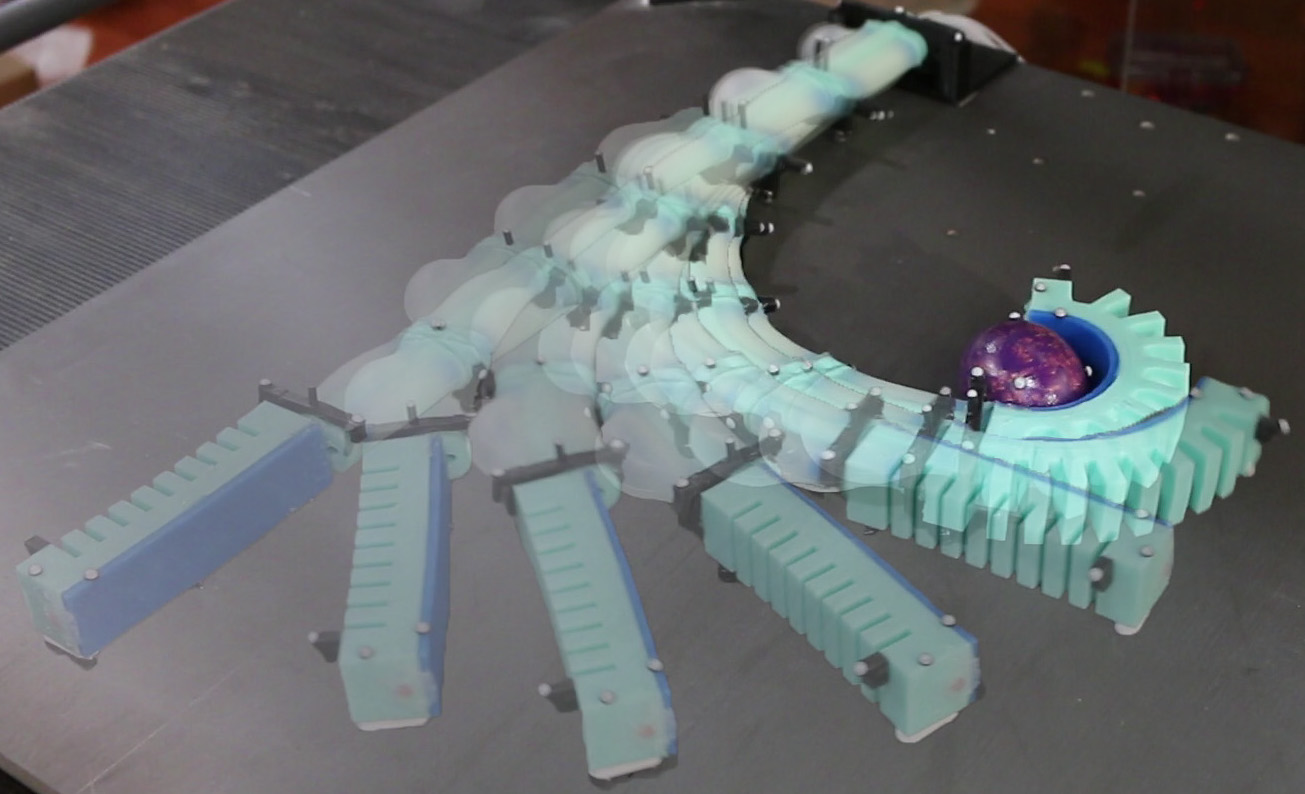
\includegraphics[width=0.9\columnwidth]{Figures/experimental_results/egg_approach/egg_approach_sequence}
   \caption{\rkk{The soft manipulator is grasping a hollowed-out egg. The robot repeatably approached, grasped and moved this delicate object without breaking it.}}
   \label{fig:egg_approach_sequence}
\end{figure}

%Challenges 
Our manipulator is highly compliant and its motion is not as precise as more traditional rigid-bodied robots. 
The control of its configuration is not only limited by the compliance of its low-pressure actuation, but also by its inherent elasticity.
%Additionally, the manipulator's compliant nature complicates the process of determining and sensing the forward kinematics.
Despite the constraints on accurate positioning introduced by the softness of the arm, we can still robustly execute autonomous grasping tasks.

%\begin{figure}[htp]
%   \centering
%   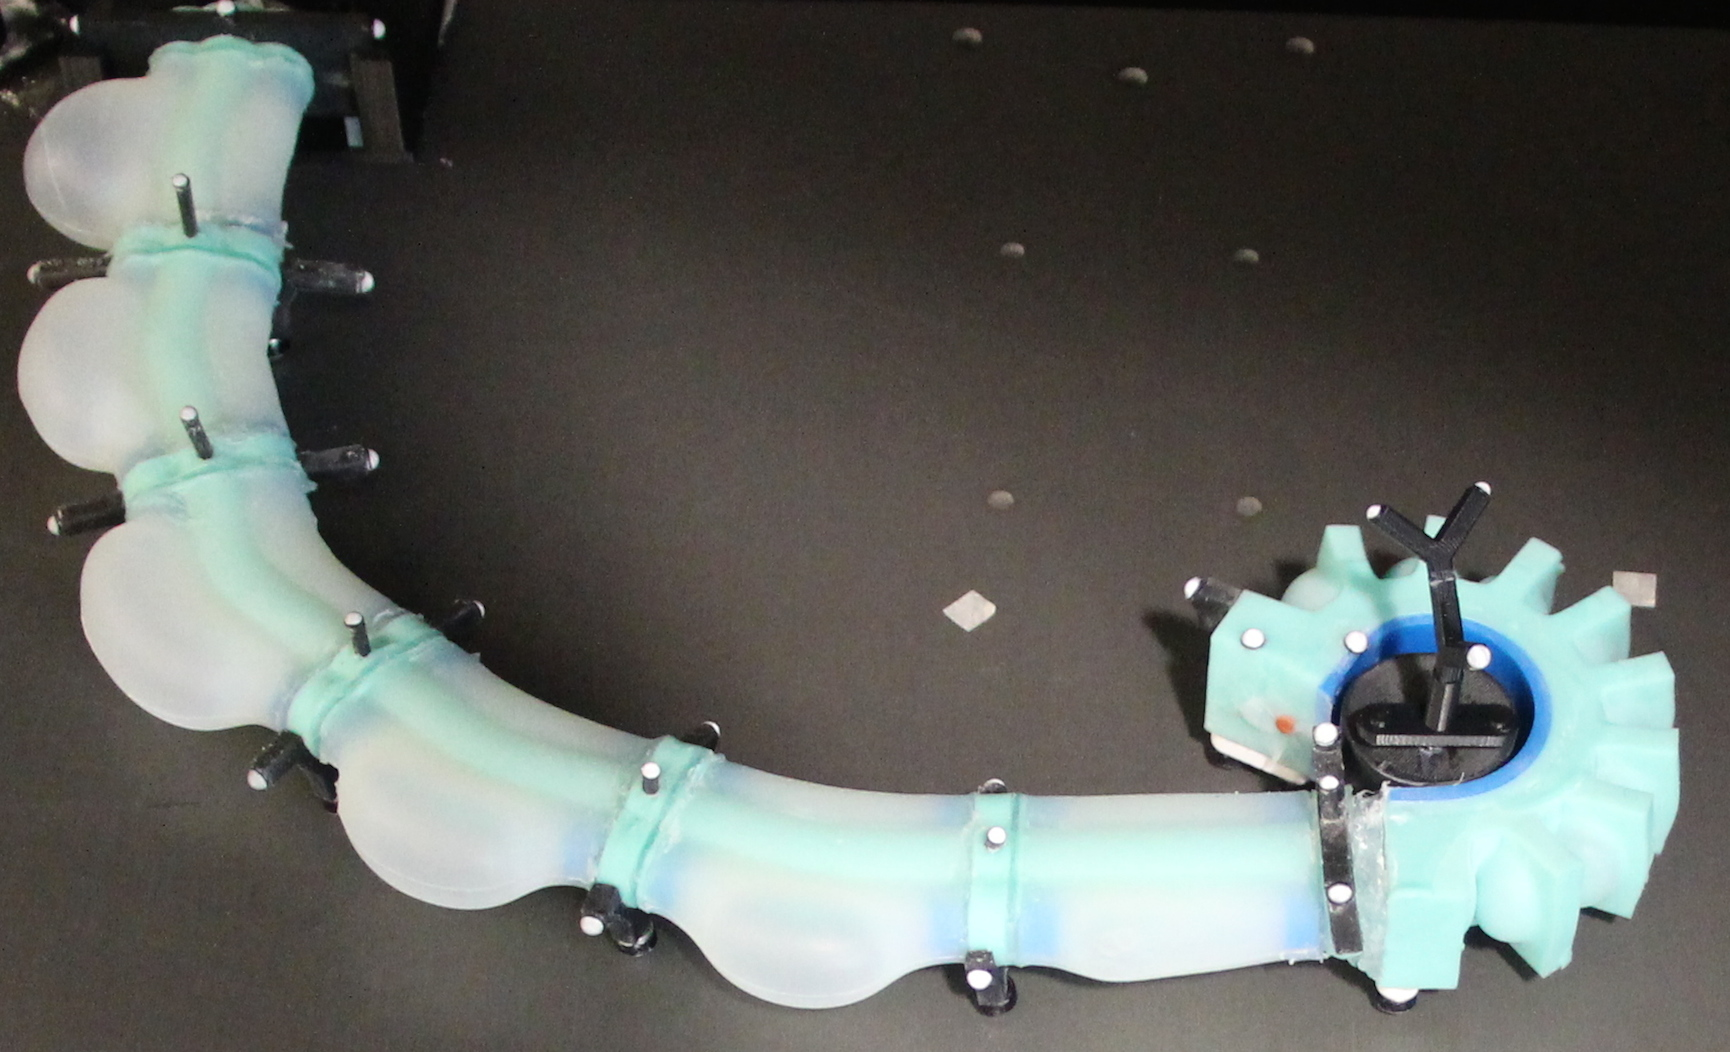
\includegraphics[width=0.7\columnwidth]{Figures/introduction/ExperimentalSetup}
%   \caption{A soft robotic arm with gripper autonomously approaching and grasping an object on a plane.}
%   \label{fig:intro}
%\end{figure}

%Our Approach
%To address these challenges, 
%\rkk{We developed planning and control algorithms for a soft robotic arm with gripper.}
\rkk{
The fluid-powered gripper at the end of the arm can grasp an object through an open-loop controlled bending motion, even if the gripper is positioned relatively inaccurately in relation to the object to be grasped.
%The gripper can conform due to his compliance to variations in object geometry, allowing it to successfully grasp.
}
The design of the gripper itself is inspired by work of Polygerinos et al.~\cite{polygerinos2013towards}
The design is advantageous for grasping, because it exhibits high curvature, minimal radial expansion, and remains compliant during actuation. 
We can repeatably fabricate the gripper using a lost-wax casting process instead of the commonly used soft lithography technique, a multi-layer lamination process.
Without weakening seams, the gripper is not prone to de-lamination under high deformations. 
By abandoning the need for a lamination process, arbitrary shaped internal channels can be achieved. 
The gripper was used as a manually actuated single finger with a bend sensor as part of a 3-fingered-hand in \cite{homberg2015haptic}.

We attach the gripper to a multi-segment soft manipulator to enable autonomous grasp-and-place capabilities on a plane. 
Positional feedback is provided in real-time from a camera system.
%and actuation of the gripper and manipulator is driven by an external fluidic cylinder array.
We present a planning algorithm that advances the arm through all necessary states of the grasp-and-place operation.
A minimal strain, collision-free approach to the object of interest is found by posing the plan as a series of constrained nonlinear optimization problems.
The system first plans concentric approach circles shrinking from the initial end-effector pose down to the object diameter.
Next, the system searches for locally optimal manipulator configurations that constrain the end-effector to lie on these approach circles, so that the manipulator does not collide with the object. 
The manipulator is then moved between these plans using closed-loop trajectories. 
After successfully approaching the object, the gripper encapsulates it.
We experimentally validate the system's ability to repeatably and autonomously grasp-and-place a randomly placed object.

\subsection{Related Work}
There are several examples of soft grippers described in recent literature, \rkk{we will mainly focus on fluidic-based systems.} 
Deimel and Brock \cite{deimel2013compliant} developed a pneumatically actuated three-fingered hand made of reinforced silicone that is mounted to a hard robot and capable of grasping.
More recently, they have developed an anthropomorphic soft pneumatic hand capable of dexterous grasps, which is not mounted to a robot, but instead just held by a human \cite{deimel2014novel}. 
Ilievski et al. \cite{ilievski2011soft} create \rkk{through a soft-lithography fabrication} a pneumatic starfish-like gripper composed of \rkk{an array of silicone chambers and a PDMS membrane.} 
\rkk{
The gripper is hanging on a string and grasps objects like an egg or a mouse in an open-loop controlled manner.
} 
Stokes et al. \cite{Stokes2014hybrid} use a soft elastomer quadrupedal robot to grasp objects in a hard-soft hybrid robotic platform. 
A puncture resistant soft pneumatic gripper is developed by Shepherd et al. in \cite{shepherd2013soft}. 
An alternative to positive pressure actuated soft grippers is a robotic gripper that makes use of granular material jamming developed by Brown et al. and detailed in \cite{brown2010universal}.
\rkk{The soft octopus-inspired arms developed in \cite{calisti2010study} and \cite{calisti2011octopus} are not fluidic powered, but instead use cables to pull rigid fixtures embedded within an elastomer body. 
The arms were capable of grasping objects like pens or screws.}
A soft robotic tentacle developed in \cite{martinez2013robotic} was able to hold a flower and a horseshoe-shaped object.
The closest related soft pneumatic actuator design to our current work is the fast Pneu-net designs by Mosadegh et al. \cite{mosadegh2014pneumatic} and by Polygerinos et al. \cite{polygerinos2013towards}.
These finger-like actuators deform with minimal volume change and can bend to high curvatures.
\rkk{None of the above described grippers were controlled autonomously to perform their tasks and accordingly no statement on repeatability of the autonomous execution was given.} 

\rkk{Cho et al. \cite{cho2009review} review several manufacturing processes for soft biomimetic robots. 
The vast majority of soft elastomer robots rely on the processes of soft lithography \cite{xia1998soft} and/or shape deposition manufacturing \cite{cham2002fast}. 
Especially noteworthy is the use of lost-wax fabrication for jammable skin chambers, which get vacuumed to stiffen up \cite{steltz2009soft}. 
The gripper presented here also uses a lost-wax molding technique, but with a different type of actuation in mind: the obtained cavity structures are inflated to cause the gripper to bend.}

%More generally, the literature has several examples of soft pneumatic elastomer robots. 
%Many of these robots use open-loop controllers. 
%There are soft fluid-powered rolling robots \cite{correll2010soft, onal2011soft, marchese2011soft}. 
%Also, there are soft-bodied robotic fish powered by pneumatics \cite{marchese2014autonomous} and hydraulics \cite{katzschmann2014hydraulic}. 
%There are soft legged pneumatic walkers \cite{shepherd2011multigait, tolley2014resilient}, explosive jumpers \cite{shepherd2013using}, and 
More recently, Marchese et al. demonstrated closed-loop position control of multi-segment soft planar fluidic elastomer manipulators in free space \cite{marchese2014design} and in confined spaces \cite{marchese2014whole}. Positioning is achieved using forward and inverse kinematic models and real-time camera measurements. 
The manipulator curvatures are controlled in real-time using a curvature-volume cascaded control law.
\rkk{The work presented in this paper builds on top of this system and expands its capabilities.
The previous version was only suitable for contactless motions in space, that would be suitable for mere inspection.
The work presented here is capable of autonomous object manipulation on a plane. 
Furthermore, this work shows that combining two different soft actuator types can leverage the strength of each and together achieve a more complicated task of manipulating objects.
The control of the arm is improved from the previous version by using a more robust vision tracking approach. 
Previously, there were only single markers along the arm, which worked for a limited motion range, but was prone to fail if the markers go out of sight or another object is introduced to the environment. 
Also, many trial runs were needed to arrive at the various final positions in the maze.
%, so the previous system was no repeatable and robust. 
}

\subsection{Contributions}
This work differs from the previous work in that we %create an entirely soft and autonomously controlled \emph{grasping} manipulation system. 
do not attach a novel soft gripper to a hard arm nor do we move the gripper around manually, but we rather take on the challenge of grasping-and-placing objects with a seven degrees of freedom planar arm made entirely from soft rubber. 
We provide in this work the following contribution to soft robotics:
\begin{itemize}
  \item \rkk{A soft manipulator consisting of a multi-segment arm with a gripper to enable fully compliant planar grasping.}
  \item \rkk{A planning algorithm to grasp-and-place randomly positioned objects on a planar surface using a 7 DOF soft manipulator.}  
  \item \rkk{Repeatable successful grasping demonstrations with a physical prototype and an experimental characterization of the uncertainty regions that can be tolerated by the soft gripper.}
  %\item \rkk{End-effector control of the grasping manipulator attached to a soft arm using a motion tracking system}.
  \item \rkk{Demonstrate that soft robots do neither require force sensing nor accurate positioning to allow for proper manipulation of delicate objects.} 
\end{itemize}

%This paper is organized as follows: In Section~\ref{sec:System_Overview} we provide an overview of the planar manipulation system. In Section~\ref{sec:soft_grasping_manipulator} the gripper morphology is described, its operating principles are discussed in relation to existing morphologies, and the lost wax fabrication process is explained. Section~\ref{sec:processing_and_control} details the planning algorithms for grasp-and-place. Section~\ref{sec:experimental_results} shows results from experimental runs and provides evaluations and experimental insights. Lastly, Section~\ref{sec:conclusion} concludes by providing a summary and discussion.



\section{System Overview}
The soft grasping manipulator shown in Figure \ref{fig:egg_approach_sequence} has six bidirectional segments with cylindrical cavities forming the arm and a single soft gripper with a pleated shape (Figure~\ref{fig:design}) as the end effector. 
The independent pneumatic actuation of the unidirectional soft gripper and each bidirectional arm segment, is achieved through an array of 13 custom fluidic drive cylinders \cite{marchese2014design}.
%All 13 cavities of the manipulator are pneumatically controlled by fluidic drive cylinders \cite{marchese2014design} and move with minimal friction on a level plane.
An object of feasible size but unknown geometry is randomly placed within the reachable envelop of the manipulator.  
The location of the manipulator and the object is determined with an external localization system. 
The motion planning algorithm as well as the curvature controller run on the control computers and take the location information as input.
The curvature controller then provides continuous closed-loop adjustment of the fluidic drive cylinder array.


%The manipulation system consists of a manipulator, a gripper, an object, a tracking system, control computers, a fluidic drive array and a rigid frame.
%The planar six segment soft rubber manipulator consists of twelve distributed elastomer actuators. 
%A soft rubber gripper is fixed to the tip of the manipulator.
%An object is randomly placed within the reachable envelop of the manipulator. 
%A motion capture system provides real-time measurements of marked points both along the inextensible back of the manipulator and on top of the object. 
%\rkk{We used the motion capture system OptiTrack Flex 3 by Natural Point, Inc.}
%The cylinder array directly actuates the manipulator and gripper.
%A rigid frame holds all the subsystems together providing reliable and consistent hardware experiments. 
%\rkk{The frame serves also as a mobile presentation platform that keeps the complete system together and holds the tracking cameras rigidly in place, not requiring recalibration after moving the system around.}


%The fluidic drive cylinders control the curvature of a bidirectional arm segment or a unidirectional gripper.
%Those cylinders are driven by a linear actuator and controlled through a motor controller, which takes its command signals from a higher-level curvature controller. 
%The design of these cylindrical actuators is given in \cite{marchese2014design}.


\section{Soft Grasping Manipulator}
\label{sec:soft_grasping_manipulator}
\rkk{The robotic manipulator is composed of multiple bidirectional planar arm segments and combined with a unidirectional soft gripper.}
%We first introduce the previously developed uniform channel design, which is used for the soft body arm segments.
%Following this, 
We describe the design, fabrication and functionality of this soft grasping manipulator. Further details on the underlying design and fabrication recipes can be found in \cite{marchese2015recipe}.

%\subsection{Uniform Channel Design of the Soft Arm}
%Several existing body segment morphologies are serpentine channels \cite{correll2010soft, marchese2014design}, uniform lateral channels \cite{marchese2014whole}, and pleated channels \cite{polygerinos2013towards, mosadegh2014pneumatic}.
%The serpentine channel design with its multiple vertical channels was first characterized by Correll et al.\cite{correll2010soft} and Onal et al.\cite{onal2011soft} and called a fluidic elastomer actuator.
%Several existing body segment morphologies are serpentine channels \cite{correll2010soft, marchese2014design}, uniform lateral channels \cite{marchese2014whole}, and pleated channels \cite{polygerinos2013towards, mosadegh2014pneumatic}.
%The serpentine channel design with its multiple vertical channels was first characterized by Correll et al.\cite{correll2010soft} and Onal et al.\cite{onal2011soft} and called a fluidic elastomer actuator.
%A cross sectional view of this design is shown in Figure~\ref{fig:design}-1.
%The design is described in \cite{marchese2014design} and paraphrased here.
%Bidirectional bending of this segment type is achieved by the pressurization of paired agonistic fluidic channel groups shown in \emph{yellow} that are separated by an inextensible but flexible constraint layer shown in \emph{black}. 
%These fluid channels are embedded within elastomer layers shown in \emph{cyan}.
%When a channel's internal fluid is pressurized, the elastomer deforms and the inextensible constraint transforms this channel deformation into segment curvature.
%The inextensible layer is typically made of a thin plastic film or fabric.
%A uniform channel design for soft segments is shown in Figure~\ref{fig:design}-1.
%It is an extension of the serpentine channel design by Correll et al. \cite{correll2010soft} and Onal et al. \cite{onal2011soft}. 
%The uniform channel design is achieved through changing both its kinematic constraints and fluidic channel geometry.
%This new design was first described in \cite{marchese2014whole} and is reused for our soft arm.
%The outer concentric layer remains composed of soft silicone rubber and is shown as \emph{transparent}.
%Bidirectional bending is achieved by pressurizing one of the two cylindrically-shaped and laterally embedded agonistic channels within this outer layer. 
%These channels are shown in \emph{yellow}.
%Also, a stiffer inner silicone layer shown in \emph{cyan} replaces an inextensible constraint layer found in the serpentine channel design.
%The stiffer inner layer introduces a partial constraint, so that an expansion of the lateral fluidic channels causes bending.
%This entirely soft design is simpler to fabricate because it does not require lamination.
%The design though is limited in defining the geometry of the fluidic channels, only cylindrical or cone shaped fluidic channels are possible. 
%This design is modular, because tubes can be passed through a hollow center, which allows the combination of many segments to an arm.
%Also, this design does not delaminate under high pressure as opposed to the serpentine design.
%This design was therefore chosen for making the arm to which the gripper is attached.

\begin{figure}[thpb]
\centering
   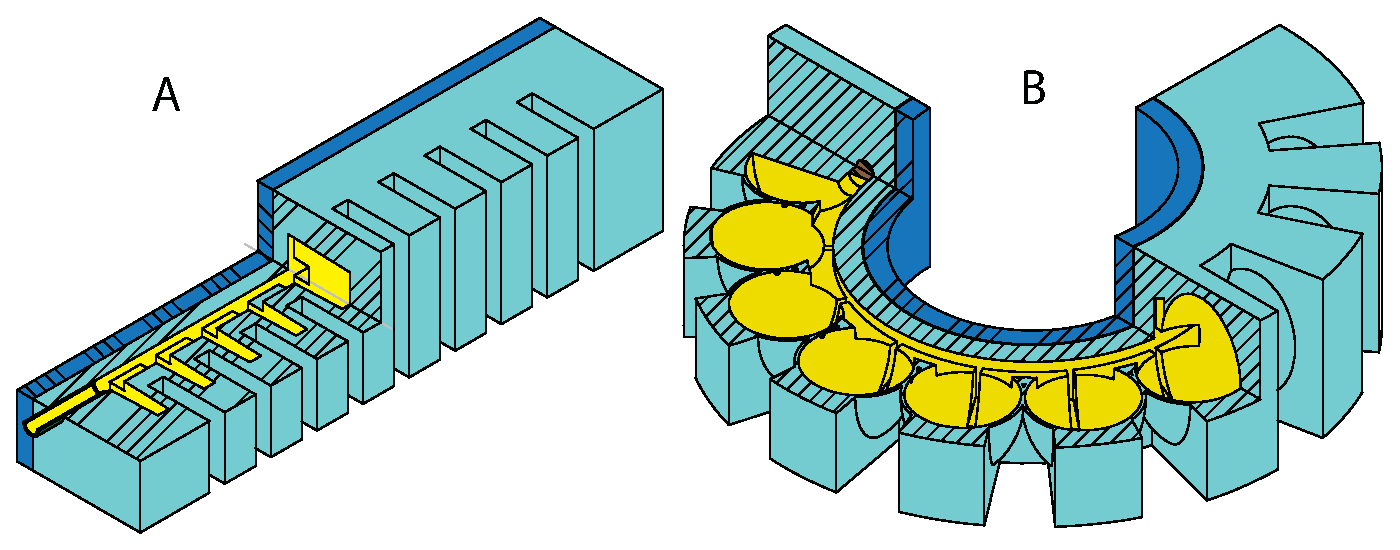
\includegraphics[width=0.90\columnwidth]{figures/robotic_gripper/design_gripper.eps}
   \caption{The pleated channel designs. (\textbf{A}) depicts the segment in an unactuated state and (\textbf{B}) shows the segment in an actuated and therefore bent state. The expansion of the pressurized channels are schematically represented. \rkk{Reproduced from \cite{marchese2015recipe}.}}
   \label{fig:design}
\end{figure}

\begin{figure}[!ht]
\centering
   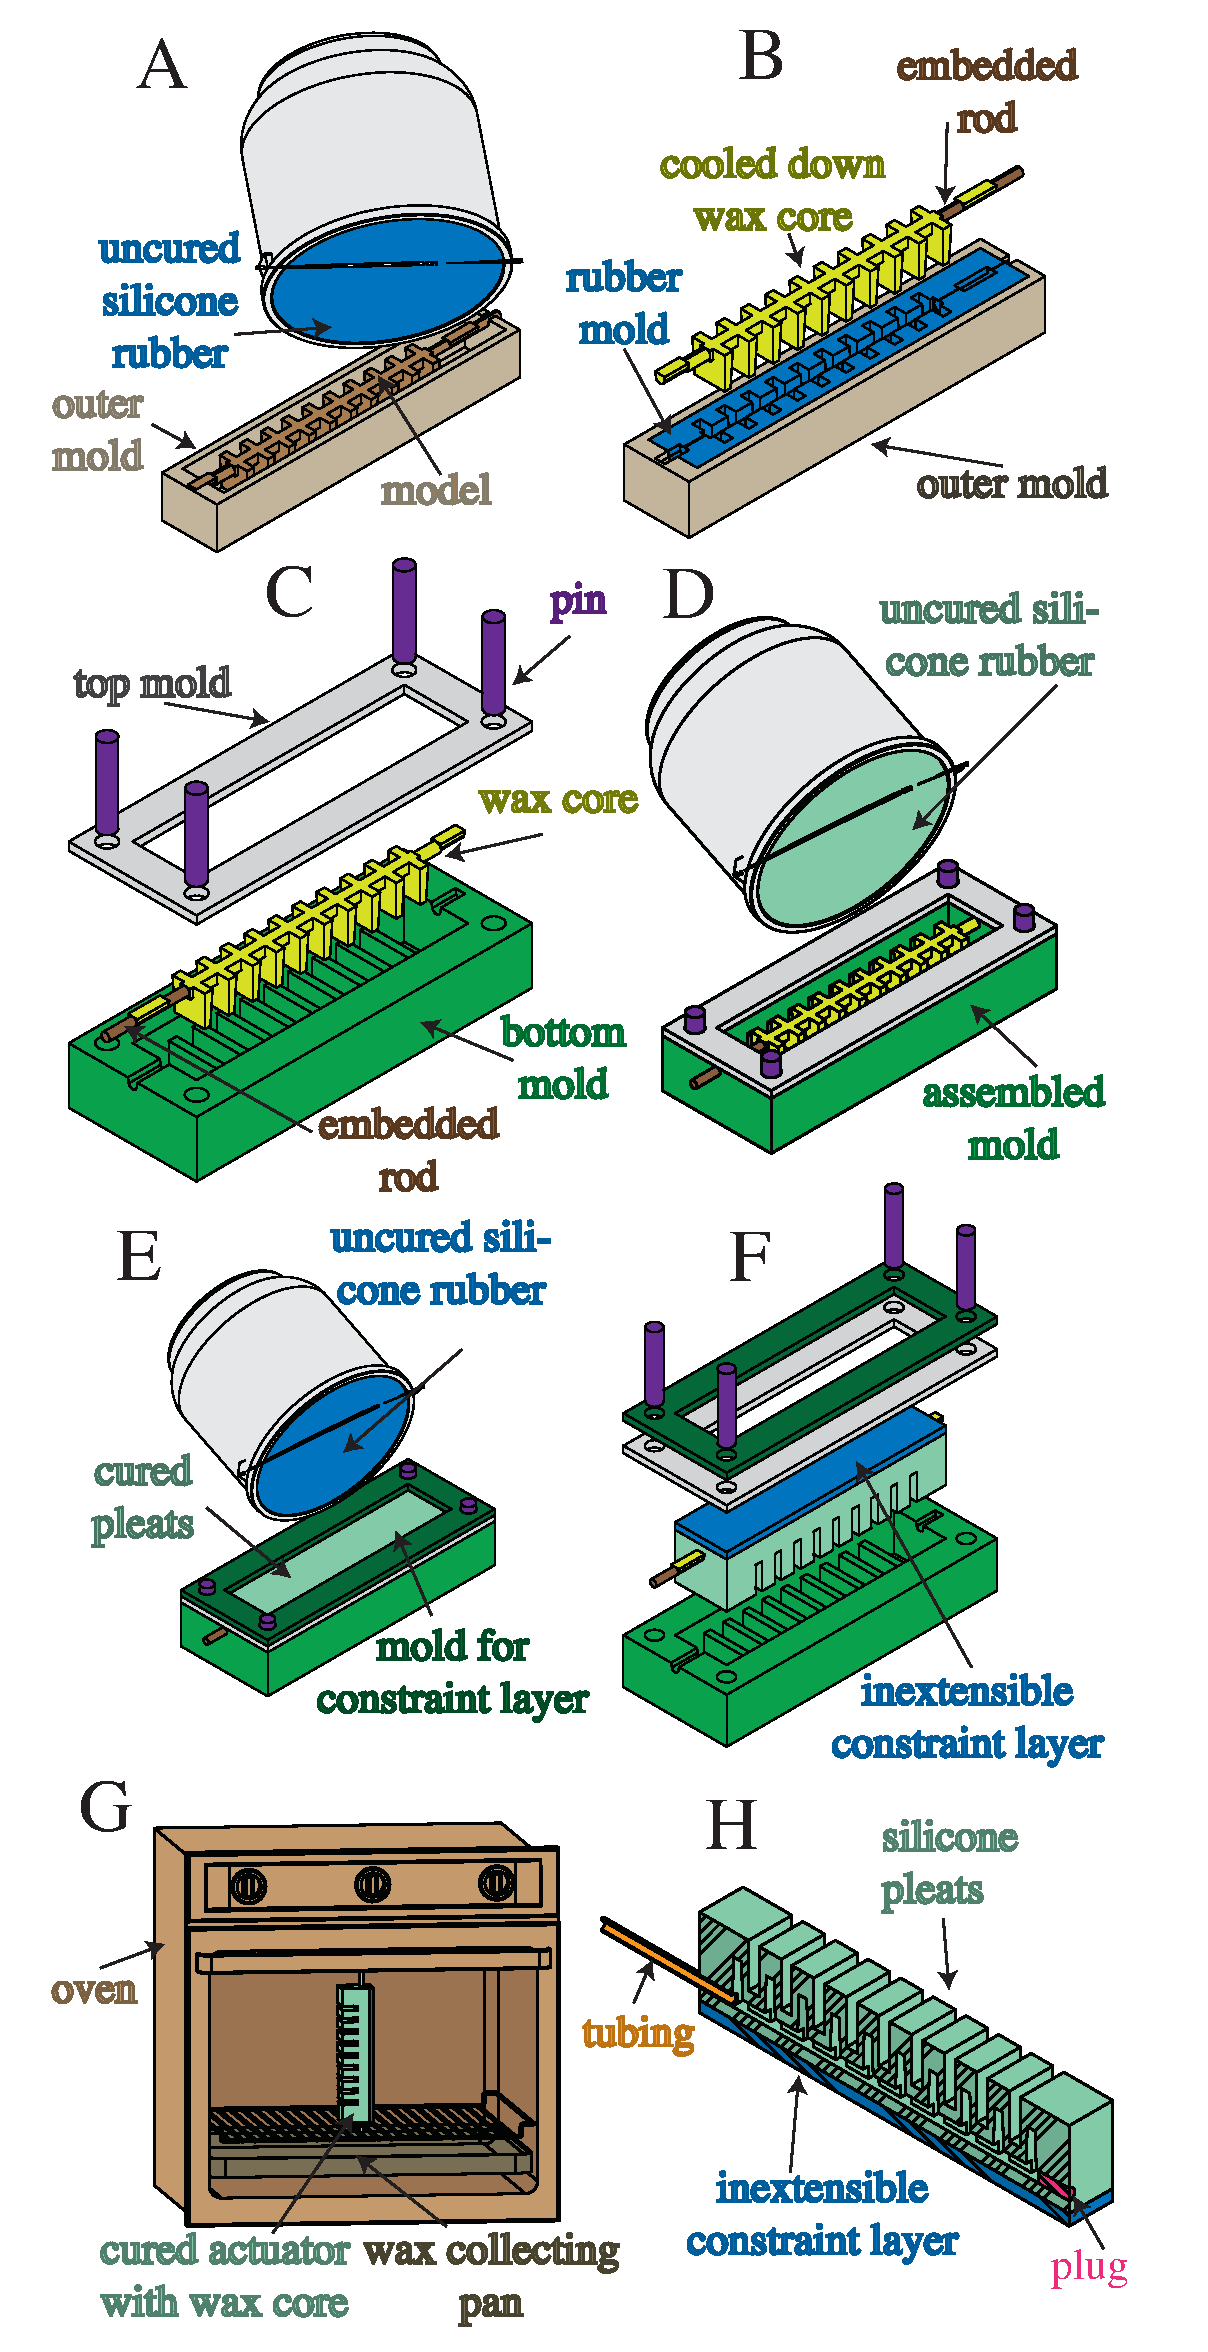
\includegraphics[width=0.85\columnwidth]{figures/robotic_gripper/fabrication_upright.eps} %fab_pleated_process_horizontal_no_labels.eps
      \caption{Gripper fabrication process. (\textbf{A}) Pour and cure a rubber mold \rkk{(blue)}, (\textbf{B}) pour wax core \rkk{(yellow)} with embedded supportive rod \rkk{(brown)}, (\textbf{C}) combine bottom mold \rkk{(green)}, top mold \rkk{(grey)} and wax core using pins, (\textbf{D}) pour \rkk{softer} rubber \rkk{(light green)} into assembled mold, (\textbf{E}) pour stiffer rubber \rkk{(blue)} on top of the cured gripper \rkk{(light green)} to form a constraint layer, (\textbf{F}) remove cured gripper from mold, (\textbf{G}) using an oven melt out wax core from the gripper, and (\textbf{H}) add silicone tubing and plug using silicone sealant. \rkk{Reproduced from \cite{marchese2015recipe}.}}
      \label{fig:fabrication}
\end{figure}

\subsection{Pleated Channel Design for the Gripper}
The pleated channel design consists of evenly spaced ribs shown in \emph{cyan} with embedded hollow sections shown in \emph{yellow}.
Cut views of the un-actuated and actuated states are shown in Figure~\ref{fig:design}.
This design approach draws inspiration for its pleats from the soft pneumatic gloves developed by Polygerinos et al. \cite{polygerinos2013towards} and its homogeneous body design is inspired from the tail design of a soft robotic fish developed by Katzschmann et al. \cite{katzschmann2014hydraulic}.
This design is advantageous for grasping because it exhibits high curvature, minimal radial expansion, and remains compliant during actuation \cite{marchese2015recipe}. 
The hollow ribs within the segment's pleats are connected by a center channel and are accessible through a front inlet.
Under fluidic pressurization of the interior channel, an individual pleat allows for a ballon-like expansion of the thin exterior skin along the axial direction.
Similar to the uniform channel design, a stiffer silicone layer shown in \emph{blue} serves as an almost inextensible constraint layer.
The sum of the ballon-like expanding motions leads to bending of the less extensible center constraint layer to form a grasp.
The pleated design is capable of unidirectional bending up to extreme curvatures.
Using a lost-wax casting approach, we are not limited in defining the geometry of the segment's fluidic channels.
Using this approach, the \emph{cyan} portion of the pleated gripper can be cured in a single step, avoiding any weakening seams due to lamination.
\rkk{Fabrication techniques based on the lamination of several cast rubber pieces lead to more manufacturing inconsistencies due to slight misalignments of layers. 
We observed that soft actuators built this way tend to rupture more easily at their weakening seams.}

\subsection{Lost Wax Fabrication for Fluidic Elastomer Actuators}
Existing soft fluidic manipulators are produced through a multi-step lamination process, which results in weakening seams that can easily delaminate. 
This limits their range of applications and lifetime.
\rkk{The retractable pin fabrication for uniform lateral channels, first introduced in \cite{marchese2014whole}, does not cause weakening seams to the actuator, but it also does not allow for cavities more complicated than cylindrical shapes.}
This is why we propose the application of lost-wax casting to the fabrication of soft fluidic actuators like a gripper.
The actuated cavities of the soft gripper are achieved by using a wax core, pourable silicone rubber and 3D printed molds.
The complete fabrication process for the soft gripper consists of eight steps that are depicted in Figure~\ref{fig:fabrication}.
The tools and equipment used are listed in Table~\ref{tab:MachineTools} and are referred to by superscripts.

In step (A), harder silicone rubber$^6$ is poured into a mold, which contains a 3D-printed model of the wax core.
In preparation for step (B), the model is removed and the rubber mold is left inside the outer mold.
A rigid rod is \rkk{embedded} as a supportive inlay inside the wax core.
The rod is laid into the cavity of the rubber mold, supported on both ends by the outer mold.
This ensures that the wax core does not break when removed from the rubber mold.
\rkk{Mold release spray is applied to the silicone rubber mold to ease the wax core removal process.}
The bees-wax$^{7}$ is heated up until it becomes fully liquefied.
The assembly of rubber mold and outer mold is then heated up for a few minutes to the same temperature as the wax.
Using a syringe, the liquid wax is injected into the assembly.
Within a few minutes, the injected wax will start to solidify and significantly shrink in volume; this is counteracted by injecting more hot wax into the solidifying wax core during cool down.
In step (B), the wax core is first allowed to completely cool down, then it is released from the mold.
In step (C), the cooled down wax core is assembled together with the bottom mold, which defines the pleated structure of the gripper.
The mold assembly is aligned with a top mold using pins. This top mold provides for additional volume to cover the wax core.
In step (D), low elastic modulus rubber$^1$ is mixed, degassed in a vacuum$^2$, and poured to form the gripper and allowed to cure.
In step (E), stiffer rubber$^3$ is poured on top of the cured gripper to form a constraint layer.
In step (F), the cured gripper is removed from the mold.
In step (G), most of the wax core is melted out by placing the gripper into an oven in an upright position.
After this, remaining wax residues are cooked out in a boiling water bath.
Finally, in step (H) a silicone tube$^5$ and a piece of silicone cord$^{8}$ get covered with silicone sealant$^4$ and are inserted into the front and back holes respectively.

\begin{table}[h]
\caption{Commercially Available Tools and Equipment}
\centering
\begin{tabular}{c l l}
\hline
\hline
\# & Product Name & Company\\
\hline
1 & Ecoflex 0030&  Smooth-On\\
2 & AL Cube & Abbess Instr. and Sys., Inc.\\
3 & Mold Star 15 & Smooth-On\\
4 & Silicone Sealant 732 & Dow Corning Corp\\
5 & PN 51845K53 & McMaster\\
6 & Mold Star 30 & Smooth-On\\
7 & Beeswax & Jacquard\\
8 & PN 9808K21& McMaster\\
\hline
\end{tabular}
\label{tab:MachineTools}
\end{table}

\subsection{Multi-segment Arm with Gripper}

The design for the arm consisting of soft cylindrical segments was described in \cite{marchese2014whole}.
\rkk{As was shown in \cite{marchese2015recipe} through the characterization of various actuator morphologies, the concatenation of soft cylindrical segments is most suitable to build up a robotic arm that can create high blocking forces per fluid energy inserted.}
 \rkk{The cylindrical segments of the arm are fabricated through a retractable pin fabrication technique, which does not require lost wax cores because of their simple cylindrical cavities.} 
Each cylindrical segment can only be actuated up to a bend angle of about $60^\circ$, therefore several segments have to be combined together to allow the arm to reach a large enough workspace to perform proper manipulation tasks on a plane. 
\rkk{Using six segments, the joint limit does not prohibit the robot to reach its own base.} %Calculating the forward kinematics, see \texttt{forwKin()} in Algorithm~\ref{alg:planGrasp}, for the 6 DOF arm with a segment length of 6.27\unit{cm} and an extreme curvature of $\kappa = \frac{60/180 \pi}{0.0627\unit{m}} = 16.7\frac{1}{\unit{m}}$ shows that the tip of the robot can reach its root at a full curl.}
The cylindrical segment design with its hollow channel in the center has enough space to accommodate for pneumatic tubes to connect to all six cylindrical segments and additionally to the pleated gripper, which is attached to the tip. 
The pleated gripper has to be appropriately sized, just big enough to allow for proper manipulation without exceeding the payload capacity of the soft arm.

\rkk{The complete multi-segment arm is supported off the ground with two roller supports per segment. 
The rollers minimize frictional forces to the surface. 
If the arm would be moved over a non-slippery surface without rollers, the frictional effects would greatly reduce the agility of the arm and largely increase the stick-slip friction effects with the ground, rendering the arm less useful.}

The independent actuation of the unidirectional gripper and each bidirectional arm segment is achieved through an array of custom fluidic drive cylinders.
%The fluidic drive cylinders control the curvature of a bidirectional arm segment or a unidirectional gripper.
Those cylinders are driven by a linear actuator and controlled through a motor controller, which takes its command signals from a higher-level curvature controller. 
The design of these cylindrical actuators is given in \cite{marchese2014design}.

\section{Planning and Control}
\label{sec:processing_and_control}
This section covers our approach to preplanning motion waypoints for the soft robot and controlling the manipulator along those points. We cover existing procedures reused within the system, and detail the system's new architecture of for performing autonomous grasp-and-place tasks, including its main component, the Grasp Object Planner.

\subsection{Existing Procedures}
The forward kinematics algorithm \texttt{forwKin()}, which we employ in this work, assumes piece-wise constant curvature according to \cite{webster2010design}. 
This algorithm was experimentally validated for the soft planar arm in \cite{marchese2014design}.
In order to uniquely fit a configuration representation to measured endpoint data in real-time, we use a previously developed single segment inverse kinematics algorithm \cite{marchese2014design} and refer to it in this work as \texttt{singSegInvKin()}.
The inputs to this block are the start and endpoint measurements in $\mathbb{R}^2$: $\mathbf{E}_n \; \forall n  = 1..N$, where $N$ is the number of segments composing the arm.
The outputs from this block are the representations of the measured manipulator configuration: $\boldsymbol{\kappa}_{\textrm{meas}}$ and $\mathbf{L}_{\textrm{meas}}$.
\rkk{Each segment of the manipulator is described by its measured curvature $\kappa_{\textrm{meas}}$ and its segment length $L_{\textrm{meas}}$}.
This work expands on the previously developed cascaded closed-loop curvature controller, whose input is target curvatures $\boldsymbol{\kappa}_{\textrm{target}}$ and whose output is the controlled adjustment of a fluidic drive cylinder array to resolve the error between $\boldsymbol{\kappa}_{\textrm{target}}$ and $\boldsymbol{\kappa}_{\textrm{meas}}$.
In this work we refer to it as the \texttt{curvatureController()}.

The planning algorithm presented in \cite{marchese2014whole} was developed to plan the motion of a soft arm  without gripper through a confined environment. 
The optimization constraints and state machine setup in that work is significantly different and not applicable to the grasping shown here. 
Therefore, a new planner is presented in the following section.

\subsection{Autonomous Grasp-and-Place System}
\label{subsec:grasp-place-planner}
The robotic manipulation system is capable of autonomously performing grasp-and-place operations. 
A state flow diagram describing its sensing, planning and executions states is given in Fig. \ref{fig:grasp-and-place-planner}. 
A motion tracker constantly captures the position of the object and passes it along to a routine, which checks for the object to settle.
\rkk{We consider the object to have settled if it has not moved by more than a small $\epsilon$ for 2\unit{s}}.
After it has settled, the Grasp Object Planner receives the coordinates and radius of the settled object and together with the current curvature values of the arm and gripper, it solves a series of constrained nonlinear optimization problems to generate end-effector poses approaching the object.
Those end-effector poses are essentially waypoints for an optimized path the robot arm should take to get to the final position without the risk of pushing away the object before the gripper arrives there. 
Forcing the arm controller to follow those intermediate waypoints ensures that the arm moves to the object while its null space maintains a convex shape, \rkk{always} bending away from the object. 
\rkk{This is a conservative approach requiring minimal computation to solve the planning problem of not prematurely colliding with the object.} 
Furthermore, \rkk{this approach} allows the arm to move in smaller portions, decreasing the risk of large overshoots due to slip-stick friction between the roller supports and the ground.
This planner is described in more detail in Section~\ref{subsec:grasp_planner}.

\begin{figure}[!htb]
\centering
   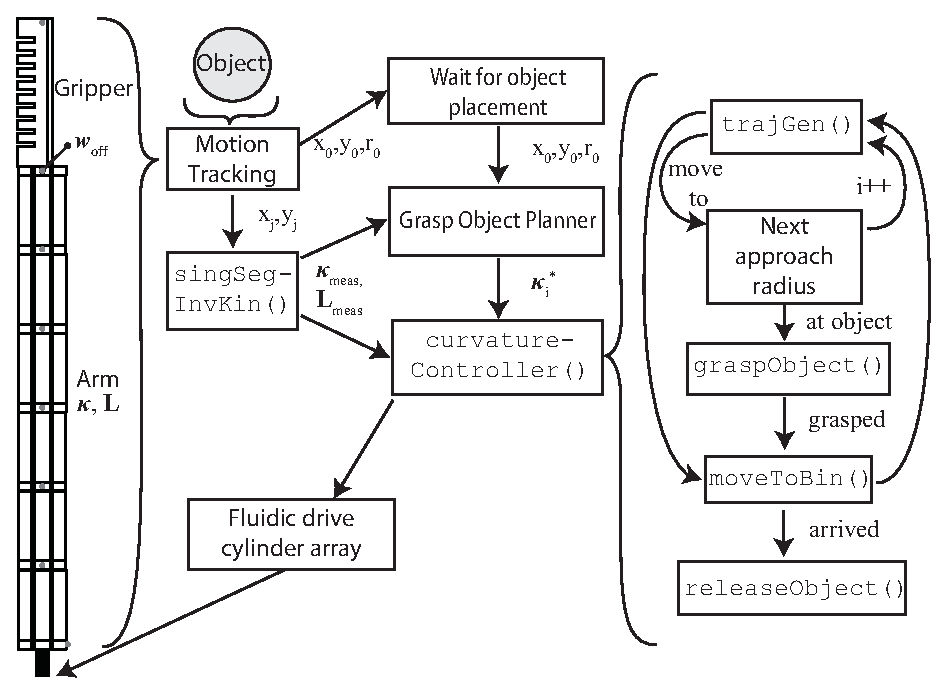
\includegraphics[width=0.95\columnwidth]{Figures/processing_control/grasp_place_planner.eps}
   \caption{State flow diagram of the grasp-and-place planner developed for the autonomous grasp-and-place operation of the manipulator. This diagram describes essentially the flow of information from the motion tracking system to the discrete hardware.}
   \label{fig:grasp-and-place-planner}
\end{figure}

The Grasp Object Planner passes the approach configurations $\boldsymbol{\kappa}_i^*$ of the arm to the \texttt{curvatureController()} for execution in real-time.
The controller receives measured curvatures $\boldsymbol{\kappa}_{meas}$ and lengths $\boldsymbol{L}_{meas}$ at an update rate of $100\unit{Hz}$ from the recursively called \texttt{singSegInvKin()} and uses these to successively control the arm to every intermediate configuration $\boldsymbol{\kappa}_i^*$.
During the arm initialization, the new curvature controller performs a pre-pressurization of both lateral channels. 
This is only done for the two segments closest to the root of the arm in order to stiffen them and shorten their response time constant.  
To allow for smoother transitions between each configuration $\boldsymbol{\kappa}_i^*$, we also added a trajectory generation procedure \texttt{trajGen()} to the new curvature controller. It generates in real-time for each individual degree-of-freedom velocity profiles with acceleration and velocity constraints.
These profiles allow real-time interpolation between the approach configurations of the arm and avoid overshooting at the next target configuration.
When the arm has arrived at the object, the curvature controller initiates \texttt{graspObject()}.
After encapsulating the object, \texttt{moveToBin()} requests \texttt{trajGen()} for another trajectory from the current pose to a pre-defined bin location.
\rkk{When the manipulator gets close to the bin location}, the procedure \texttt{releaseObject()} causes the gripper to open and release the object.

\subsection{Grasp Object Planner}
\label{subsec:grasp_planner}
A fundamental component of the grasp-and-place system is its ability to plan a feasible approach motion to the object.
That is, given the location $\left(x_o, \, y_o\right)$ and radius $r_o$ of a round object as well as the manipulator's current configuration $\boldsymbol{\kappa}_{\textrm{meas}}$ \rkk{and segment lengths $\mathbf{L}_{\textrm{meas}}$}, we determine a series of locally optimal manipulator configurations $\boldsymbol{\kappa}_i^* \; \forall i \, = 1.. numMoves$ that will, if sequentially achieved, bring the manipulator gradually closer to the object while any part of the arm is not touching the object.

We refer to these as approach configurations.
The process for determining these approach configurations is detailed in the \texttt{planGrasp()} procedure within the Grasp Object Planner, see Algorithm \ref{alg:planGrasp}.
The planner is visualized in Figure \ref{fig:planGrasp}.
In short, we define a series of approach radii $r_{a_i} \;  \forall i\, = 1.. numMoves$ that define concentric \rkk{green} circles shrinking from the manipulator's starting tip pose towards the center of the object.
Given actuator limits, we then search for a series of feasible manipulator configurations $\boldsymbol{\kappa}_i^*$ that will place the robot's end-effector on these \rkk{green} circles, parameterized by $r_a$ and $\phi$, while minimizing manipulator deformation.
\rkk{Minimized manipulator deformation is chosen as the optimization criterion, because it is proportional to the energy consumed by the fluidic drive cylinders and it also minimizes the strain to the soft actuators.}

\begin{figure}[htpb]
\centering
   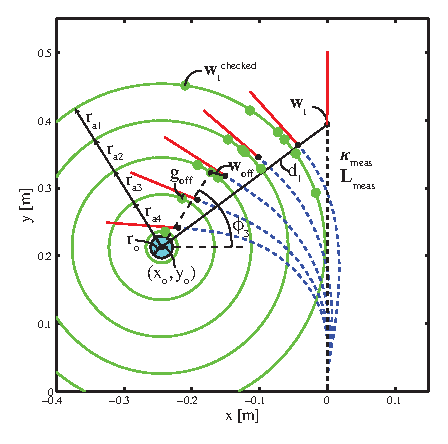
\includegraphics[width=0.85\columnwidth, trim = 0mm 0mm 5mm 5mm, clip]{Figures/processing_control/grasp_object_planner.eps}
   \caption{Visualization of the Grasp Object Planner. Concentric approach circles are shown in \emph{green} and are centered about the object shown in \emph{cyan}. The locally optimal approach configurations are shown in \emph{blue} and the gripper is shown in \emph{red}. The initially measured manipulator configuration is shown in black.}
   \label{fig:planGrasp}
\end{figure}

\begin{algorithm}[!htbp]
\begin{small}
  \SetAlgoLined\DontPrintSemicolon
  \KwIn{
  $\boldsymbol{\kappa}_{\textrm{meas}}$, $\mathbf{L}_{\textrm{meas}}$ $\gets$ measured arm configuration \;
  $\boldsymbol{\kappa}_{\textrm{off}}$ $\gets$ \rkk{measured manipulator} configuration at start \;
  $g_{\textrm{off}}$ $\gets$ gripper offset normal to end-effector\;
  $x_o$, $y_o$, $r_o$ $\gets$ object center coordinates and radius \;
  $N$ $\gets$ number of manipulator segments}
  \SetKwFunction{planGrasp}{planGrasp}
  \SetKwFunction{findOptimalConfig}{findOptimalConfig}
  \SetKwFunction{forwKin}{forwKin}
  \SetKwProg{myproc}{Procedure}{}{}
  \myproc{\planGrasp{}}{
  $\mathbf{w}_t \gets \forwKin \left( \boldsymbol{\kappa}_{\textrm{meas}}, \, \mathbf{L}_{\textrm{meas}}, \, N, \, L_N \right)$. \;
  $d_1 \gets \| \left[ x_o, \, y_o \right]^{\textrm{T}} \, - \, \mathbf{w}_t \|$. \;
  $d_2 \gets d_1 - r_o - g_{\textrm{off}}$. \;
  $numMoves \gets \lfloor \frac{d_2}{\Delta d} \rfloor$. \;
  $i$ = 0. \;
  \Repeat{$i$ = $numMoves$}{
    $i$ = $i \, + \, 1$ \;
    $r_{a_i} \gets d_1 \, - \, i\,\frac{d_2}{numMoves}$. \;
    $\boldsymbol{\kappa}_i^* \gets$ \findOptimalConfig{$r_{a_i}$}\;
  }
  \KwRet{$\boldsymbol{\kappa}_i^* \quad \forall i \, = 1.. numMoves$} \;}{}
  \setcounter{AlgoLine}{0}
  \SetKwProg{myproc}{Procedure}{}{}
  \myproc{\findOptimalConfig{$r_{a_i}$}}{
  $\begin{aligned}
    & \boldsymbol{\kappa}^* \, \gets \, \underset{\phi, \, \boldsymbol{\kappa}}{\text{min}}
    & & \mathbf{R} \, \left( \boldsymbol{\kappa} \, - \, \boldsymbol{\kappa}_{\textrm{off}} \right)^2. \\
    & \text{subject to}
    & &  \mathbf{w}_t \gets \begin{bmatrix} x_o \, + \, r_{a_i} \, \cos{\phi} \\ y_o \, + \, r_{a_i} \, \sin{\phi} \\ \phi \, + \, \frac{\pi}{2} \end{bmatrix}. \\
    & & & \mathbf{f} \gets \forwKin\left( \boldsymbol{\kappa}, \, \mathbf{L}, \, N, \, L_N \right). \\
    & & & \mathbf{w}_t - \mathbf{w}_{\textrm{off}}\left(r_o, \, \phi \right) - \mathbf{f} \, = \, \mathbf{0}. \\
    & & & \kappa_{n}^{\text{min}} \leq \kappa_n \leq \kappa_{n}^{\text{max}} \quad \forall \, n = 1 \, .. \,N. \\
    \end{aligned}$ \;
  \KwRet{$\boldsymbol{\kappa}^*$} \; }
  \setcounter{AlgoLine}{0}
  \SetKwProg{myproc}{Procedure}{}{}
  \myproc{\forwKin{$\boldsymbol{\kappa}$, $\mathbf{L}$, $i$, $s$ }}{
  \KwIn{$\boldsymbol{\kappa}$, $\mathbf{L}$, $i$ the segment of interest index, $s$ the arc length along the indexed segment}
  \eIf{$i = 0$}{
        $\theta_{i}(0) \gets \theta_0(0)$. \;
        $x_{i}(0) \gets 0$.\;
        $y_{i}(0) \gets 0$.\; }
    {
        $\left[ x_{i}(0), \, y_{i}(0), \, \theta_{i}(0) \right] \gets \forwKin \left(\boldsymbol{\kappa}, \, \mathbf{L}, \, i-1, \, L_{i-1} \right)$.\;
    }
    $\theta \gets \theta_{i}(0) + k_i s$. \;
    $x \gets x_{i}(0) + \frac{\sin{\theta}}{k_i} - \frac{\sin{\theta_{i}(0)}}{k_i}$. \;
    $y \gets y_{i}(0) - \frac{\cos{\theta}}{k_i} + \frac{\cos{\theta_{i}(0)}}{k_i}$. \;
  \KwRet{$\left[ x, \, y, \, \theta \right]^{\mathrm{T}}$ or $\left[ x, \, y \right]^{\mathrm{T}}$}}
  \caption{Grasp Object Planner}
  \label{alg:planGrasp}
\end{small}

\end{algorithm}

The procedure \rkk{\texttt{planGrasp()} in Algorithm \ref{alg:planGrasp}} first determines the manipulator's current tip pose $\mathbf{w}_t$ and the Euclidean distance $d_1$ between the tip and the object's center. 
\rkk{The arc length input to the arm's forward kinematics is the $N$-th element of the segment lengths $\mathbf{L}_{\textrm{meas}}$.}
\rkk{The end effector offset $\mathbf{w}_{\textrm{off}}$ describes the distance from the root of the gripper, to an offset point close to the lower end of the gripper's palm. It is visualized in the top left corner of Fig.~\ref{fig:grasp-and-place-planner}.}
\rkk{The length} $\mathbf{g}_{\textrm{off}}$ represents the component of the end effector offset $\mathbf{w}_{\textrm{off}}$, which is normal to the end effector orientation. 
The minimal tip transit distance $d_2$ is calculated by \rkk{considering the object's radius $r_o$ and the gripper normal offset $\mathbf{g}_{\textrm{off}}$.} 
Also, the number of approach configurations $numMoves$ is determined as $\lfloor \frac{d_2}{\Delta d} \rfloor$, where $\Delta d$ is an allowable incremental distance. 
Using these parameters, approach radii $r_a$ \rkk{shown by the green circles} are iteratively calculated and their corresponding locally optimal configurations are found \rkk{by using the optimization equation and constraints described in procedure} \texttt{findOptimalConfig($r_{a_i}$)} \rkk{of Algorithm \ref{alg:planGrasp}}.

\rkk{The procedure \texttt{findOptimalConfig($r_a$)}} is posed as a nonlinear optimization \rkk{problem}. 
Here, the objective function represents the summation of independently weighted manipulator curvatures \rkk{$\boldsymbol{\kappa} - \boldsymbol{\kappa}_{\textrm{off}}$.}
\rkk{The weights are set by the matrix $\mathbf{R}$.}
\rkk{The variables to optimize for are $\phi$ and $\kappa$.}
The optimization constraints \rkk{cause} the manipulator's tip to lie on and to be tangent to the approach circle. 
\rkk{The constraints also ensure that the manipulator segment curvatures do not exceed the single soft actuator limits.}
\rkk{Furthermore,} this \rkk{procedure} leverages the arm's forward kinematics \texttt{forwKin()} defined in \cite{marchese2014design} and reproduced \rkk{in the last section} of Algorithm~\ref{alg:planGrasp} for convenience. 

\rkk{The nonlinear optimization problem was implemented using Matlab’s Optimization Toolbox with the function calls \emph{fmincon}, which finds the minimum of a constrained nonlinear multivariable function. Sequential Quadratic Programming was used as the solver with a relative upper bound of $2 \times 10^{-3}$ on the magnitude of the constraint functions. The lower bound on the size of a step was given by $1 \times 10^{-6}$. The solver takes about 1\unit{s} on a regular PC to solve for all waypoints from start to finish.} 

\section{Experimental Results}
\label{sec:experimental_results}
In the following section summarizes the results from experiments with the soft manipulator. We discuss the grasping of delicate objects and cylindrical objects as well as the repeatability and success rate of the autonomous system.
 
\subsection{Aggregate System}
\label{sec:aggregate_system}
The aggregate \dr{soft manipulation} system is shown in Figure~\ref{fig:sys_overview}.
%The planar six segment soft rubber manipulator consists of twelve distributed elastomer actuators. This manipulator moves with minimal friction on a level plane.
%A soft rubber gripper is fixed to the tip of the manipulator.
As our localization system, the OptiTrack Flex 3 by Natural Point provides real-time measurements of marked points both along the inextensible back of the manipulator and on top of the object. 
A rigid frame holds all the subsystems \rkk{as a mobile presentation platform} together providing reliable and consistent hardware experiments without the need for recalibration.

\begin{figure}[htbp]
\begin{centering}
  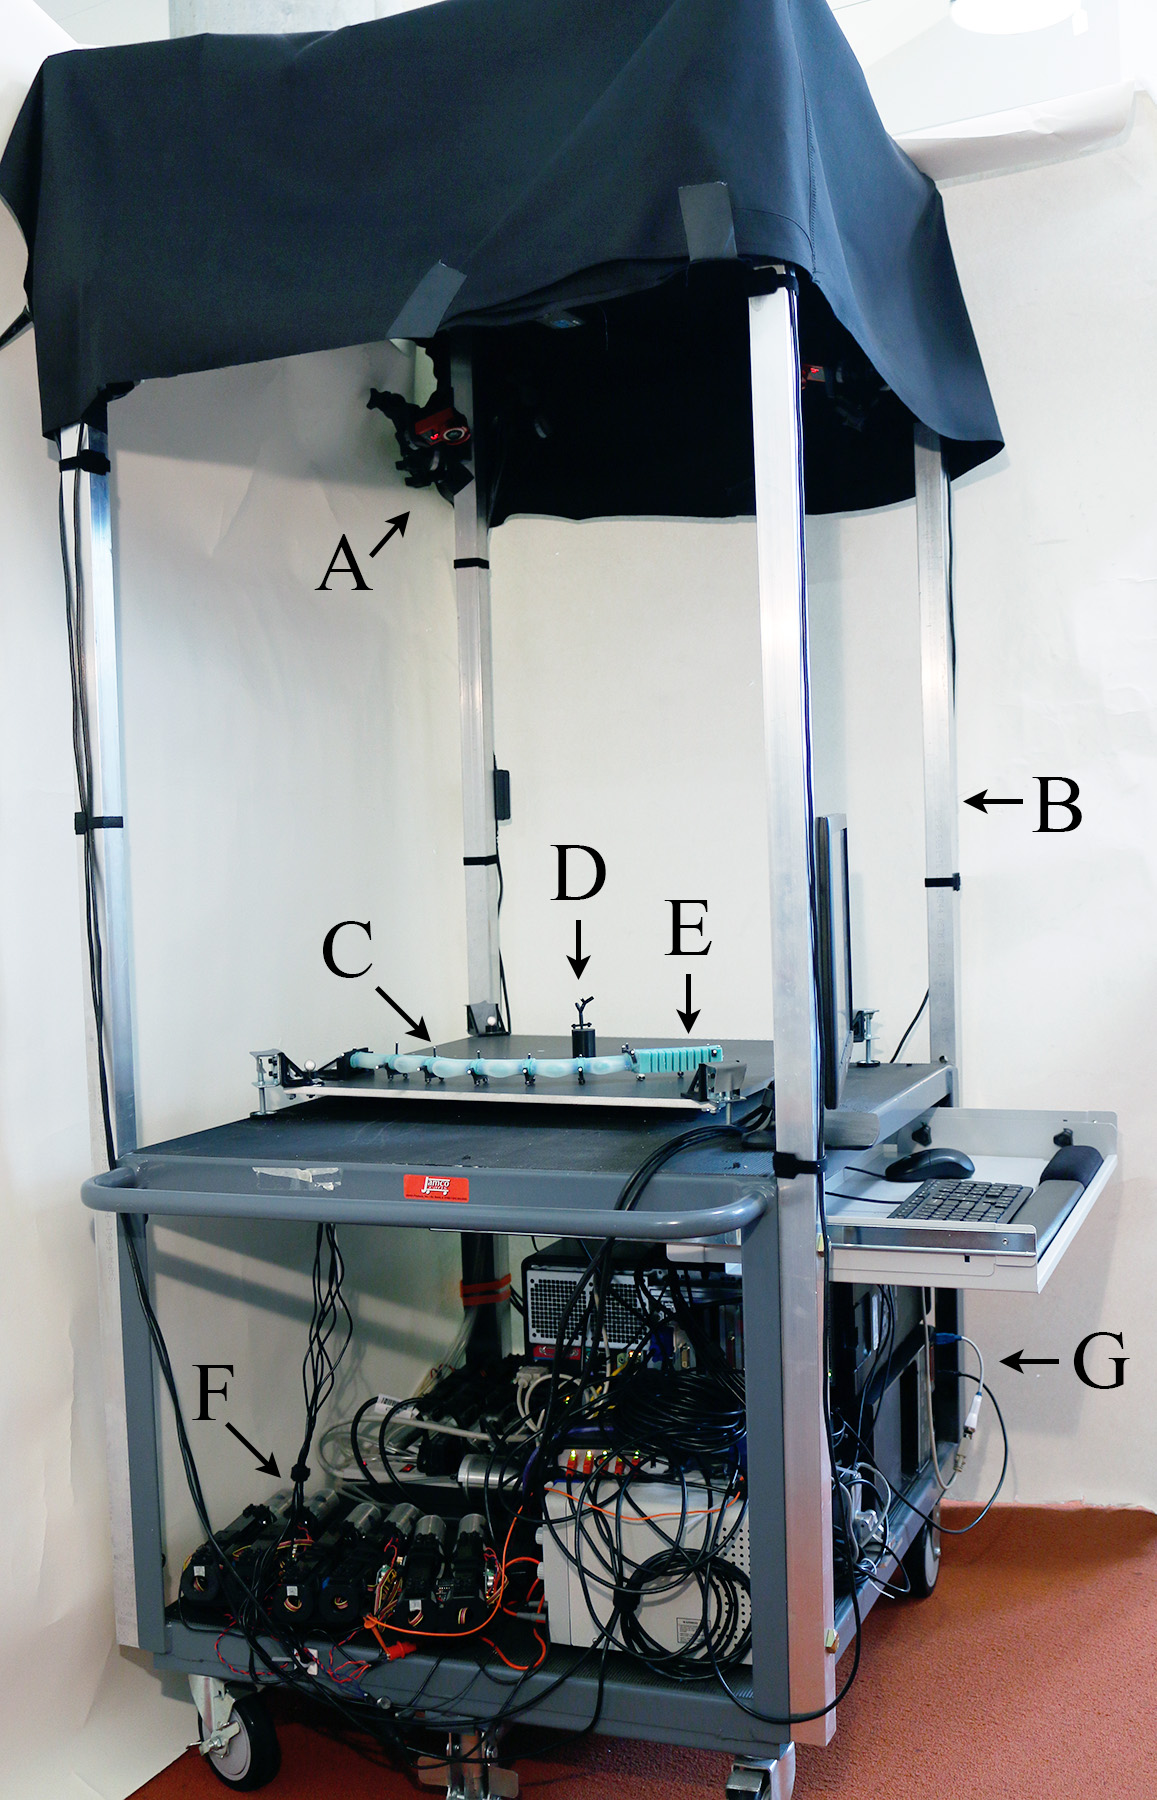
\includegraphics[width=2.0in]{Figures/system_overview/sys_overview_smaller}\\
  \caption{System Overview. The system is composed of (\textbf{A}) a motion capture system, (\textbf{B}) rigid frame, (\textbf{C}) soft six segment planar manipulator, (\textbf{D}) an object within the grasp envelope, (\textbf{E}) a soft gripper fixed to the manipulator, (\textbf{F}) a fluidic drive cylinder array to control actuation, and (\textbf{F}) computers for real-time processing and control.} \label{fig:sys_overview}
\end{centering}
\end{figure}


\subsection{Grasping Delicate Objects}
\rkk{It was shown in \cite{marchese2015recipe} that pleated grippers of similar dimensions like the one used in this work can be contiuously actuated in a pressure range of 0-60\unit{kPa} and create blocking forces in the range of 0-2\unit{N}. This fine actuation range and the fact that soft manipulators easily conform to shapes implies that grasping delicate objects should be possible.}
The manipulator in fact picks up delicate objects \rkk{such as eggs, shuttlecocks or bakery items} without \rkk{squishing} or breaking those. 
Figure~\ref{fig:egg_approach_sequence} shows \rkk{for example} how the manipulator approaches and grasps an egg.
Delicate objects can be manipulated without requiring a shape or a force sensor within its structure, since the compliant gripper body conforms to the object.
Rigid-bodied grippers usually rely on force sensing or another type of sensory feedback to avoid damage caused to the object.

\begin{figure}[htb]
\centering
   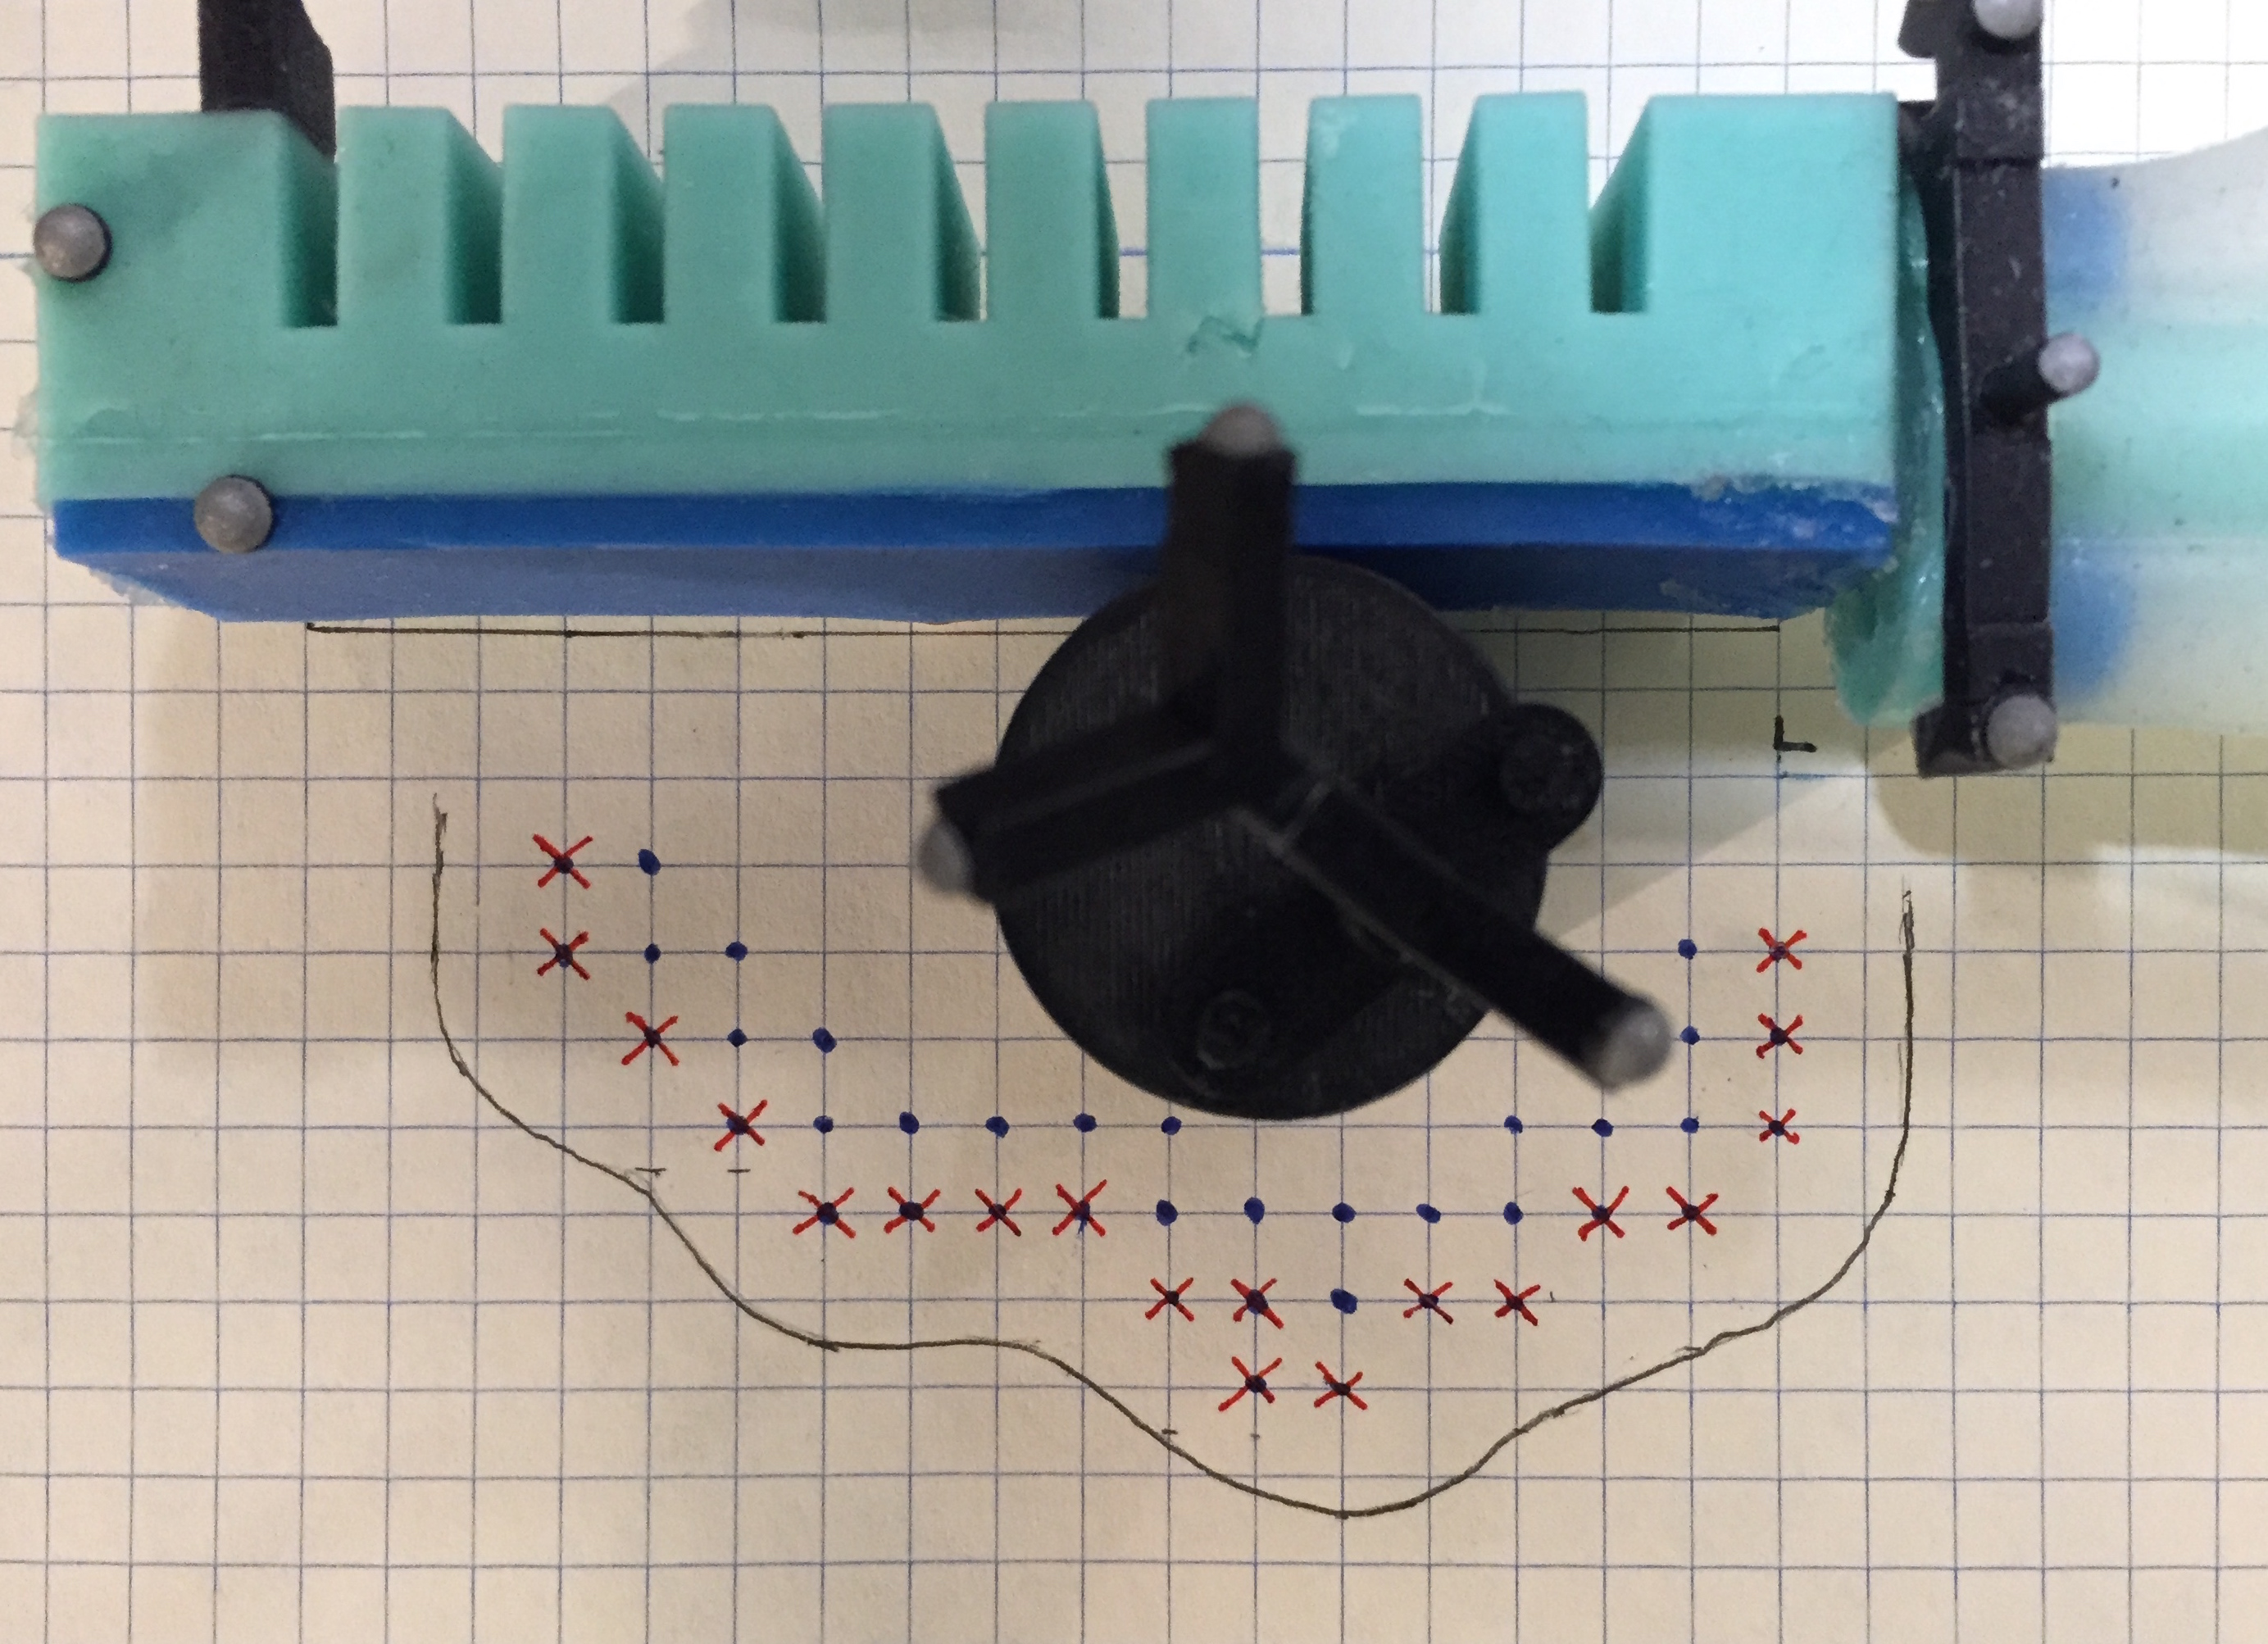
\includegraphics[width=0.8\columnwidth]{Figures/experimental_results/uncertainty}
   \caption{Experimental characterization of the gripper's capture region: the allowable positioning uncertainty is determined through repeated placements of the center of a cylindrical object at different points on a grid relative to the gripper. Blue dots indicate all object center positions for which a grasp could be performed successfully, red crosses show the positions where a grasp failed. The grey line outlines an area for the object to be positioned within so the gripper can grasp it. The evaluation of the capture region was performed similarly to a method described in \cite{dogar2010push}.}
   \label{fig:grasp_uncertainty}
\end{figure} 

\subsection{Repeated Grasp Experiments}
We performed 25 experimental grasp-and-place trials at various positions to demonstrate the capabilities and repeatability of our system.
The results of all the trials are shown in Figure~\ref{fig:allTestsOverlaid}.
One representative approach, grasp, and retract move is shown in Figure~\ref{fig:oneTrialVsTime}.
In 23 of 25 experimental trials, the manipulator successfully achieved the task of grasping an object and bringing it to a bin location shown in red.
\rkk{The test object has a weight of 18\unit{g} and a diameter of 3.3\unit{cm}.}
The object was placed five times on each of the five points marked on the board.
The markers only serve as a reference point for the user to place the object roughly at the same point at every repetition.
The user's placing accuracy is not important to the algorithm, \rkk{since the tracking system newly registers the position of the object every time it is placed.}
The five points were chosen to approximately represent the major portion of the manipulator's reachable workspace.
As long as the root of the gripper stops so that the object is located within the capture region, the gripper will pick it up through its sweeping closing motion. The capture region is shown in grey in Figure~\ref{fig:grasp_uncertainty}. 

The evaluation of the capture region is performed similarly to a method described in Dogar and Srinivasa\cite{dogar2010push} work on determining capture regions for a push-grasp of a classical robotic gripper.
\rkk{Grid paper and fine markings on all four sides of the round object ensure that the placement by the user is accurate within $\pm$1\unit{mm} in relation to the discrete placement locations on the grid. This test serves as a qualitative measure to show qualitatively a relation between object size to gripper size to area of successful grasp.}
\rkk{This characterization was repeated two times, resulting always in the same capture region.}
Despite positioning inaccuracies of the soft manipulator, the gripper can nevertheless successfully perform a grasp of an object. 

When the arm reaches \rkk{its straight pose within a relatively large delta}, it drops the object.
\rkk{For these experiments, we focus on showing the capability of picking up objects at various places and moving them around, there is no emphasis set on having to drop off the object at a specific pose. To indicate that the arm can move the object after grasping, the arm was controlled to go back to the fully straight pose. When it got fairly close to that final straight pose within a large allowable delta, the gripper was set to release and drop the object. It was not ensured by the planner that the arm had to first settle to zero velocity at the final straight pose. As a consequence of this, the experimental data indicates as a red bin a relatively wide drop off area.}

\begin{figure*}[htbp]
\begin{centering}
  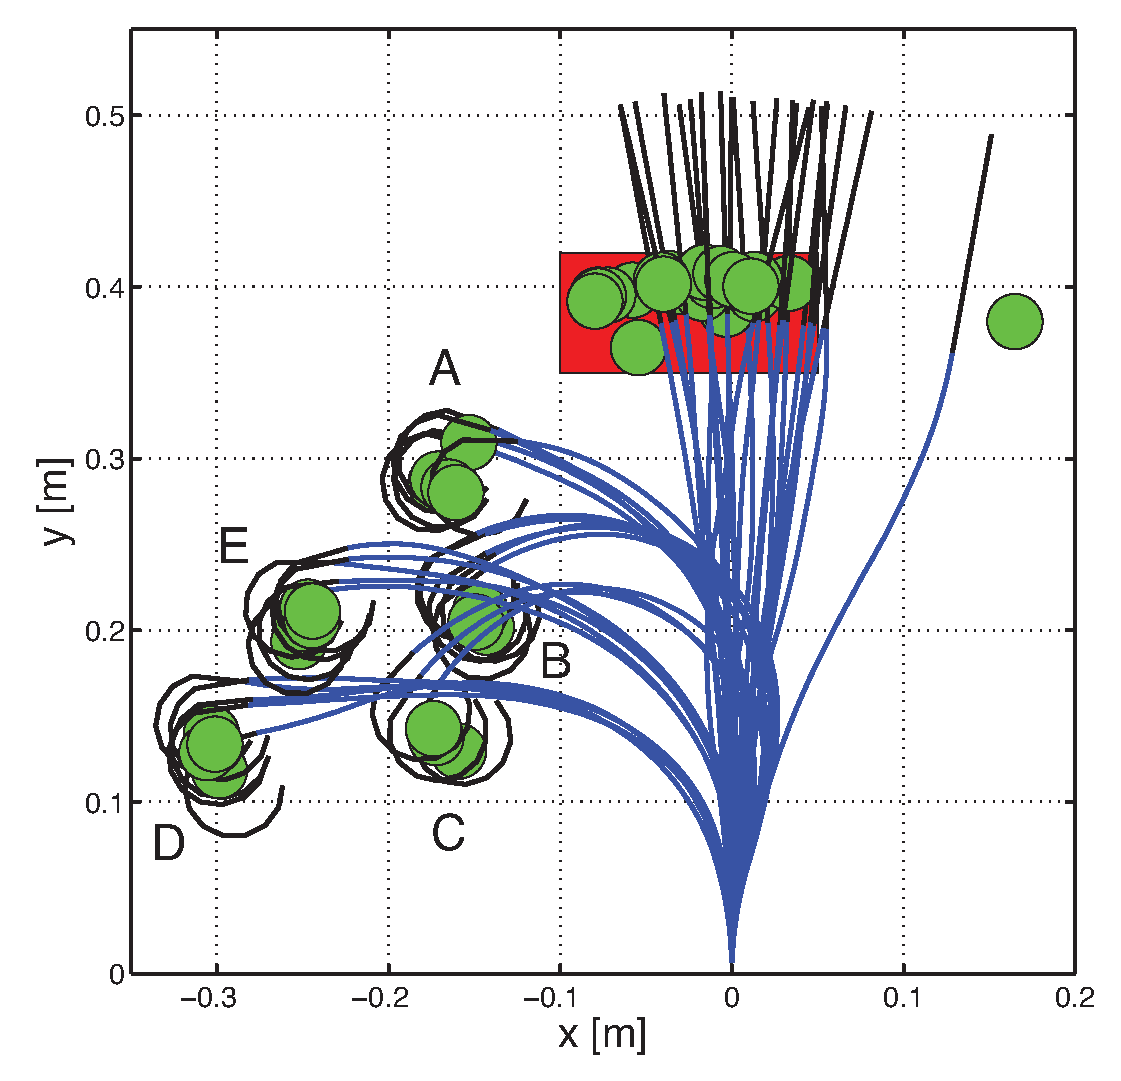
\includegraphics[width=0.5\textwidth]{Figures/experimental_results/allTestsOverlaid.eps}
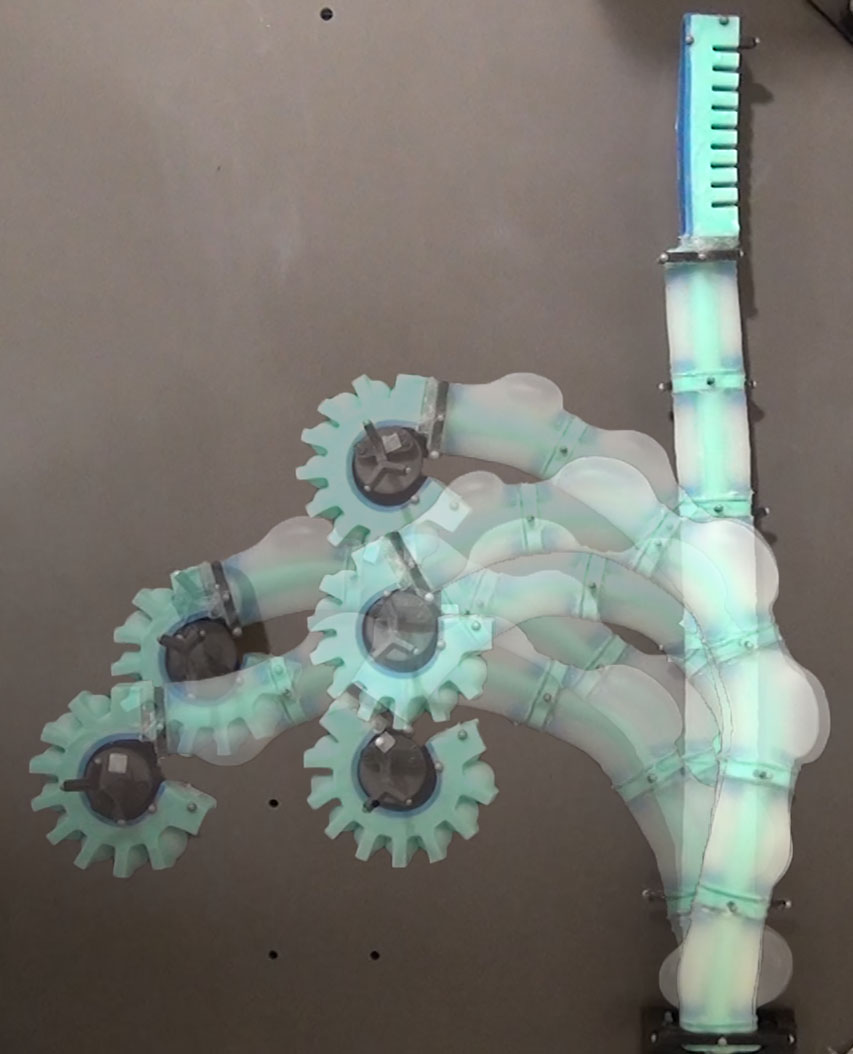
\includegraphics[width=0.385\textwidth]{figures/experimental_results/five_grasps.jpg}
\caption[Left: All 25 experimental grasping trials.]{Complete set of experimental grasp-and-place trials. In these experiments, the arm moves from an initial straightened configuration to grasp a round object placed in one of five locations (A-E). The arm then returns the object to a bin location shown in red. For each trial, a seven degrees of freedom manipulator representation is generated at both the \emph{grasped} and \emph{released} state using experimental data and is shown in blue. The corresponding 1 degree-of-freedom end-effector representation is shown in black. The round object's measured position at each state is shown in green. Right: Overlaid photographs of the manipulator grasping an object placed at each of the five locations. }\label{fig:allTestsOverlaid}
\end{centering}
\end{figure*}

The unsuccessful trials happened due to stick-slip friction between the roller bearings and the table surface.
Our kinematic modeling does not account for this non-linear behavior, which acts as a disturbance and can lead to failure to arrive at the next waypoint.
To be more specific, in one of the trials, the robot slowed down too much before it almost reached its next waypoint and because of friction the arm halted to a full stop. 
The proportional gain of the curvature controller was not able to compensate for that small positional delta and since the relatively low saturation level of the integrator portion of the controller was saturated, the arm did not move to the next waypoint pose. 
It is to note, that the saturation level for the integrator is defined by a safety limit on the maximal inflation of the robotic arm.
In the other unsuccessful trial, the stick-slip friction also caused the arm to halt before a waypoint. The controller built up enough forcing due to inflation, so that the arm slipped over the close waypoint without having all of its single arm segment curvature within an acceptable epsilon.
The controller then tried to swing back to fulfill the missed waypoint, missed it again and that finally caused the whole arm to oscillate back-and-forth and eventually push the object off the table.
In one of the other trials, the grasp and return was successfully performed, but a small overshoot over the final bin location at the end of the return caused the arm to drop off the table, which could have been avoided if the table would have not been too small towards the right.
This outlier is shown in Figure~\ref{fig:allTestsOverlaid}.
Overall, the experiments show that the system was repeatably able to autonomously locate a randomly placed object within its workspace, plan the arm motions, and perform the task of grasping and placing the object.

\subsection{Experimental Insights and Limitations}
The system can drag payloads of less than 40\unit{g}, higher payloads cause the cylindrical arm segments to stall and possibly lift off the table without moving the payload.
There is a trade-off between the reachable workspace and the maximum payload.
As the length of the arm increases, more workspace can be reached while less payload can be manipulated. 
Most of the payload capability is already used up by the attached gripper itself.
A smaller gripper would allow for larger payloads to get picked up, but consequently only smaller objects can be grasped.
The workspace of the manipulator is limited to the top and left by the maximal extension length of the arm, and to the bottom by the maximum bending curvature, which the arm can achieve without over-actuating a single segment.
\rkk{The gripper presented can not only pick up a round object, but also more arbitrarily shaped objects of similar size, for example a star-shaped object, a tape holder, a shuttlecock or an egg.}
Objects were only grasped within the left quadrant of the arm, because of the gripper orientation and an upright initial starting pose.
\rkk{A smoothing of the complete trajectory with several intermediate waypoints was found to be necessary. The amount of intermediate waypoints is determined by the variable $\Delta d$, which we found empirically to be 5\unit{cm}, around half the length of the gripper. A new waypoint is sent to the controller immediately after arriving within a small delta of the previous waypoint, the controllers for each arm segment then compensate for the new delta in curvature as quickly as possible to get to the new pose $\kappa_i^*$.}
\rkk{The instabilities observed in the unsuccessful trials could be solved by loosening the constraints on the planner. The planner could allow the arm controller to have the arm pass over each intermediate waypoint without having to get to a full stop within an arbitrarily chosen delta of curvature values. The planner could take as a measure of progress a decreasing cartesian distance of the gripper to its final target pose.}
\rkk{We developed an end-to-end system that can approximately locate an object placed at an a priori unknown location and move it somewhere else. The external localization system is a convenient way to approximately identify the location of the object and to track how the object is moved around.
The exteroceptive tracking system has the disadvantage that the full occlusion of one or more markers can cause the tracking system to temporarily loose track of a measured arm segment. 
In that case, the control loop can not function properly until the occlusion disappears. 
The external localization system could be replaced with another method for localizing the manipulator and the object in the workspace.
For example, proprioceptive sensors within the segments could solve this issue partially. 
A first step towards proprioceptive sensing was done for three soft fingers arranged as a hand in \cite{homberg2015haptic}.}

\begin{figure*}[htbp]
\begin{centering}
  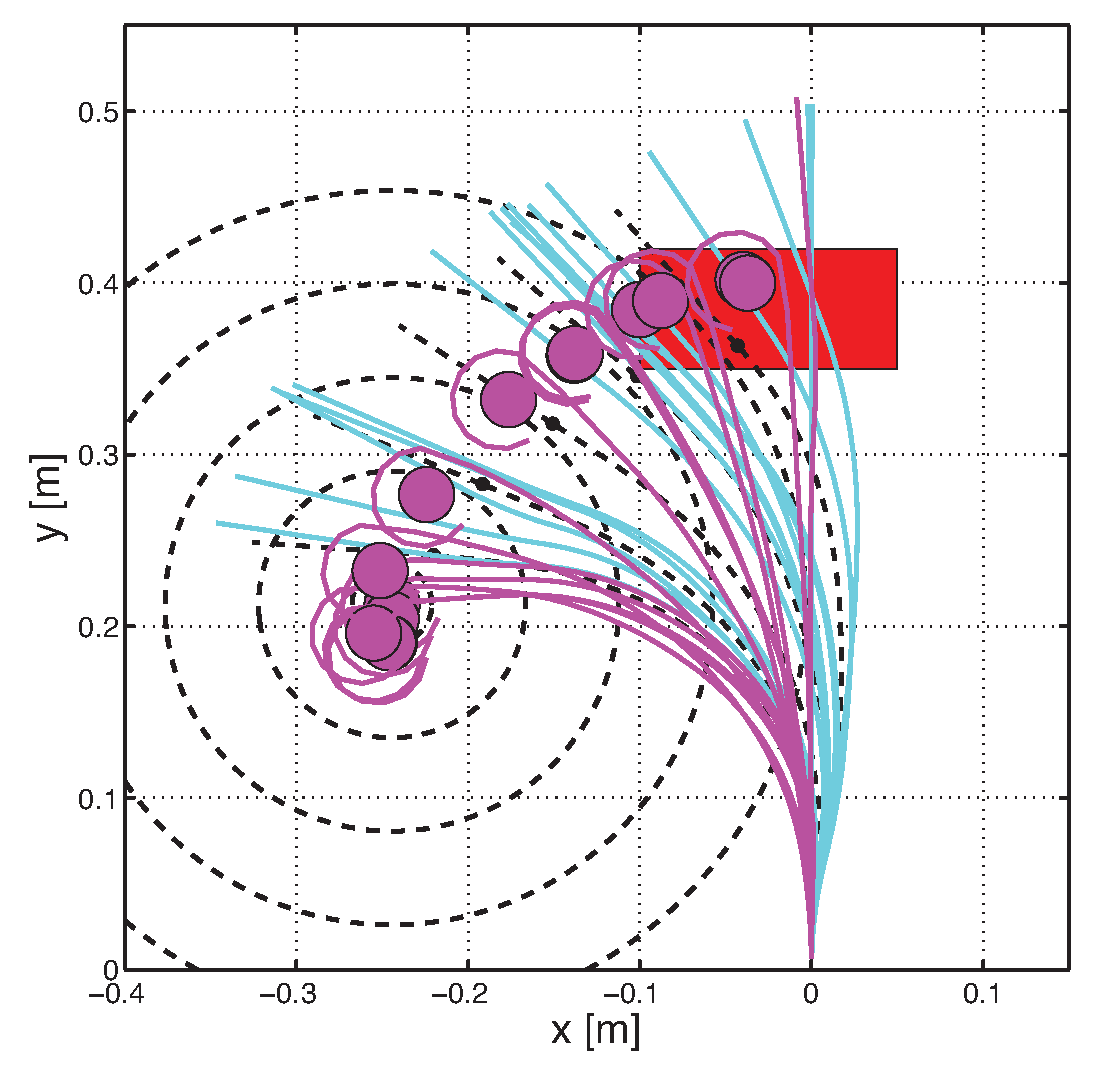
\includegraphics[width=0.375\textwidth]{Figures/experimental_results/oneTrialVsTime.eps}
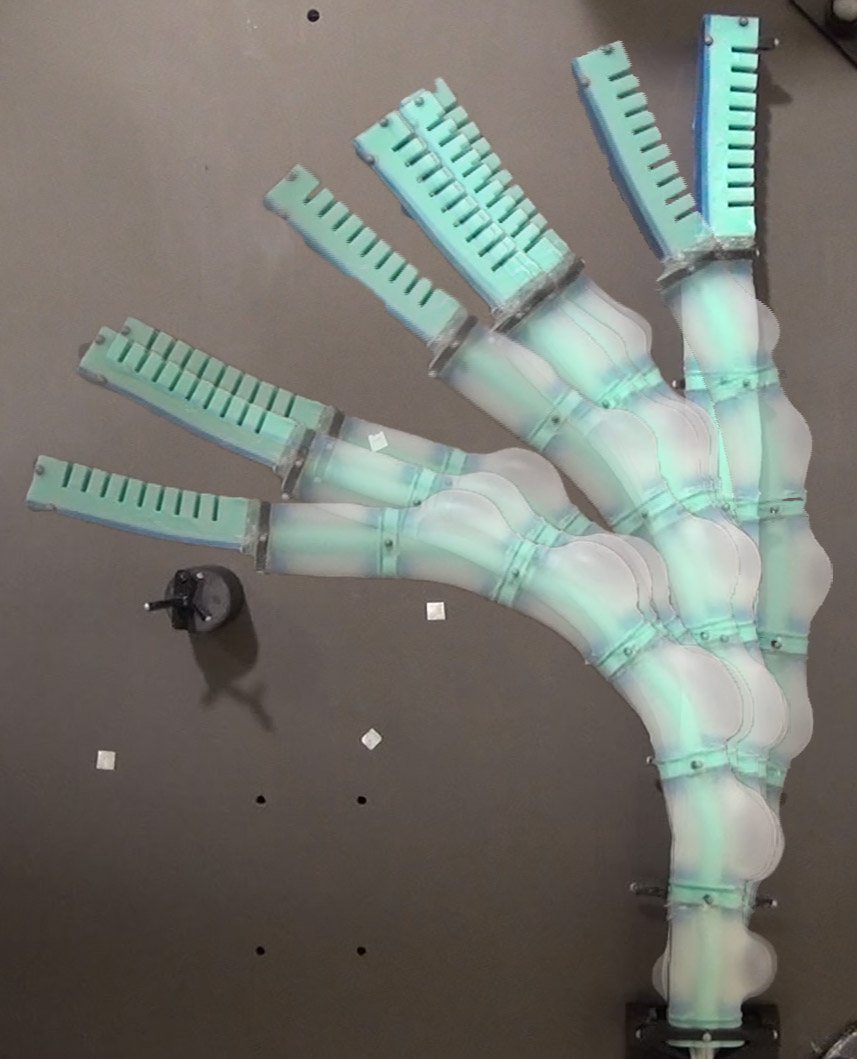
\includegraphics[width=0.30\textwidth]{figures/experimental_results/exp5a-4_sweep_to_object.jpg}
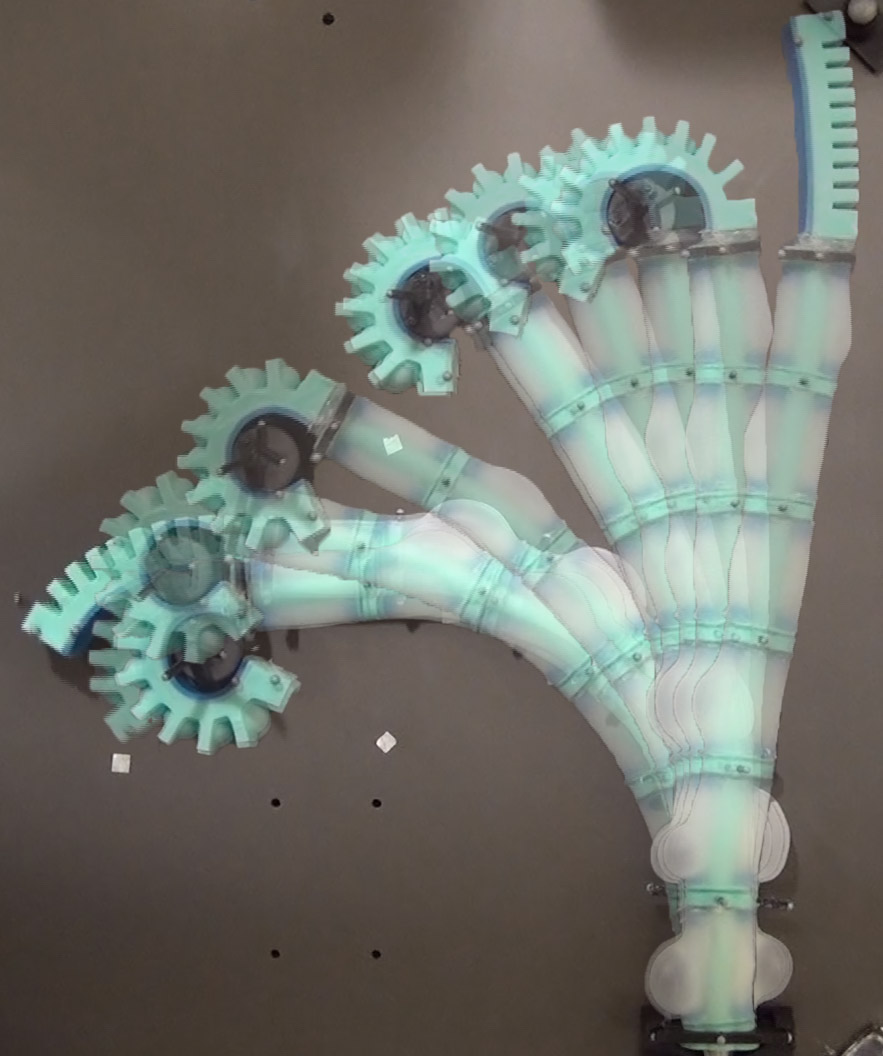
\includegraphics[width=0.31\textwidth]{figures/experimental_results/exp5a-4_sweep_to_bin.jpg}
  \caption{Left: A time series representation of an experimental grasp-and-place trial for an object located at point E. Here, the locally optimal planned manipulator configurations as well as planned sequential approach circles are shown as black dotted curves. The arm and gripper are shown in their experimentally determined configuration representations at 1 second intervals. The cyan configurations represent the manipulator prior to grasping the object, that is moving from its initial configuration to the object's location. \rkk{Depending on where the object is placed, the arm takes between 17-35\unit{s} to approach it.} The magenta configurations represent the manipulator after grasping the object, that is moving from the object's location back to the bin location shown in red. \rkk{This task of moving back to the bin takes between 10-20\unit{s}.} Right: A photograph of the arm moving from its initial pose to the object and from the object to the release location, respectively.}
\label{fig:oneTrialVsTime}
\end{centering}
\end{figure*}

\rkk{The experiments were performed for picking up objects on the left quadrant of the manipulator.
Grasping objects on both sides of the manipulator could be achieved in various ways by 
\begin{enumerate}
\item replacing the large gripper at the end of the arm with two smaller grippers next to each other, 
\item mounting roller supports on the top face of the manipulator and then rotating the manipulator at its root by $180^{\circ}$,
\item increasing the reachable workspace through starting the soft arm at an extreme curvature configuration within the right quadrant.  
\end{enumerate}
}

\section{Conclusion}
\label{sec:conclusion}
This work introduced a new manufacturing approach for a soft manipulator and demonstrated its capabilities through autonomously grasping-and-placing a randomly positioned object.
To produce the complete soft manipulator used, an entirely soft gripper was designed and fabricated and then combined with a previously developed soft robotic arm.
It was then shown that a minimal strain and collision-free approach to an object of interest can be achieved by posing the grasp motion plan as a series of constrained nonlinear optimization problems.

The fabrication approach presented has potential to generalize beyond just the fabrication of a gripper.
The new approach is advantageous because it allows for arbitrary designs of internal fluidic cavities and the casting of a homogeneous soft segment. It removes the need for laminating several separately casted parts together.
Such a homogeneous soft segment is less prone to rupture and to manufacturing inconsistencies, and would therefore allow for better robot performance.

The manipulator is suitable to perform delicate tasks with low payloads, for example grasping objects that should not be squeezed and/or should not break during manipulation.
\rkk{The ability to successfully and repeatedly perform object manipulation using a fully soft, multiple degree of freedom arm suggests} that despite their extreme compliance, soft robots are capable of \rkk{reliable and robust} object manipulation while simultaneously providing inherently safe interactions with the environment.
We \rkk{also} demonstrated the \rkk{manipulator's} ability to autonomously grasp an object, which leads to many potential applications \rkk{for full soft robotic manipulation}.
\rkk{In a manufacturing setting, this could resemble a soft robot stretched widely to pick up objects situated at various locations.}
In a human-centric environment, soft arm grasping manipulation may enable soft robots to interact safely with humans.
Furthermore, in a surgical setting, highly compliant soft robots with grippers may assist with operations in sensitive environments during tasks where no high level of precision is required.
\rkk{To foster those assumptions, future work could investigate the dexterity of the arm when approaching same object poses in various ways, just by changing the constraints and cost function when optimizing for the inverse kinematics solution.
Integrating proprioceptive sensing within a multi-segment soft actuator will further improve the use of these manipualtors in occluded environments.}



\section*{ACKNOWLEDGMENTS}
This research was conducted in the Distributed Robotics Laboratory at MIT with support from the National Science Foundation, grant numbers NSF 1117178, NSF IIS1226883 and NSF CCF1138967, and National Science Foundation Graduate Research Fellowship Program, primary award number 1122374. We are grateful for this support.


\bibliography{katzschmann2015autonomous}

\end{document}
